\documentclass[11pt]{article}
\usepackage[utf8]{inputenc}
\usepackage{amssymb}
\usepackage[left=1.5in,right=1.5in,top=1.5in,bottom=1.5in]{geometry}
\usepackage{graphicx}
\usepackage{fancyhdr}
\usepackage[hyphens]{url}
\usepackage[hyperfootnotes=false]{hyperref}
\usepackage[font=small,labelfont=bf]{caption}
\usepackage{svg}
\usepackage{caption}
\usepackage{subcaption}
\usepackage[noadjust]{cite} % to cite in ranges
\usepackage{titlesec}

\title{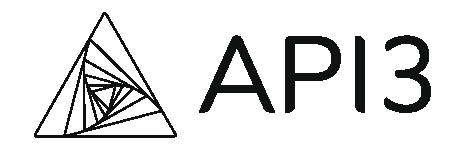
\includegraphics[width=0.7\textwidth]{fig/api3/api3} \\ Decentralized APIs for Web 3.0}
\author{Burak Benligiray, Sa\v{s}a Mili\'{c}, Heikki Vänttinen}
\date{\href{https://api3.org}{api3.org} \\ \medskip September 2020, v1.0.0}

% no paragraph indents
\setlength\parindent{0pt}
% vertical paragraph spacing
\setlength{\parskip}{1em}
% add dot after section number
\titlelabel{\thetitle.\quad}

\pagestyle{fancy}
\fancyhf{}
\lhead{\small API3: Decentralized APIs for Web 3.0}
\rhead{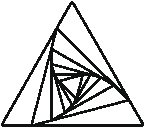
\includegraphics[height=7mm]{fig/api3/api3-solo}}
\fancyfoot[C]{\thepage}

\begin{document}

\pagenumbering{gobble}

\maketitle

\begin{abstract}
\noindent 
With decentralized applications beginning to provide meaningful services in areas such as decentralized finance, there is an increasing need for these applications to receive data or trigger events using traditional Web APIs.
However, the generic oracle solutions fail to appropriately address the API connectivity problem due to an over-generalized and misguided approach.
To remedy this issue, API3 will drive a collaborative effort to create a new generation of blockchain-native, decentralized APIs, or dAPIs for short.
dAPIs are composed of first-party oracles operated by API providers, and thus are more secure and cost-efficient than alternative solutions that employ middlemen.
At the core of the governance, security, and value capture mechanics of this initiative will be the API3 token.
Staking the token will grant its holders full governing rights over the API3 DAO along with all the associated rewards.
Staked API3 tokens will be used as collateral for the on-chain insurance service that will provide quantifiable and trustless security guarantees to dAPI users.
These mechanics will remove the need for a central authority at the ecosystem level.
As a result, the API3 Project will allow smart contract platforms to leverage APIs for the building of meaningful applications in a truly decentralized and trust-minimized way.
\end{abstract}

\newpage
\pagenumbering{roman}
\setcounter{page}{2}
\renewcommand{\contentsname}{} % no "contents" title
\tableofcontents


\newpage
\pagenumbering{arabic}
\setcounter{page}{1}

%~~~~~~~~~~~~~~~~~~~~~~~~~~~~~~~~~~~~~~~~~~~~~~~~~~~~~~~~~~~~~~~~~~~
\section{Introduction}
\label{sec:introduction}

We are witnessing the birth of decentralized applications that are able to interact with the real world, which is immediately reflected in the value they capture.
The most prominent example of this phenomenon is the recent surge of value flowing into DeFi (decentralized finance) with more than \$8B total value locked in various applications as of September 2020~\cite{defipulse}.
A DeFi application typically requires asset prices to be delivered to its smart contract platform through a data feed~\cite{liu:2020}.
This data feed facilitates the application’s interaction with the real world, ultimately allowing it to provide meaningful services such as derivative exchanges and lending.
What is unfolding right now is not only the rise of DeFi but the rise of decentralized applications that can meaningfully interact with the real world, and DeFi is only the tip of the iceberg.

Businesses offer a wide variety of services over Web APIs, ranging from providing asset price data to executing traditional financial transactions.
It is critical for decentralized applications to be able to access the kind of services that Web APIs offer in order to interact with the real world, yet these APIs are not natively compatible with decentralized applications.
Existing middleman-based interfacing solutions are centralized, insecure, and expensive; and are only being used for lack of a better alternative.
With API3, we aim for the concept of an API to take the next evolutionary step to meet the inevitably strict decentralization requirements of Web~3.0 without employing third-party intermediaries.
We will be using the term dAPI to refer to this new generation of decentralized APIs.

A dAPI is a secure and cost-efficient solution to provide a traditional API service to smart contracts in a decentralized way.
It is composed of the following elements:
\begin{itemize}
    \item multiple APIs, where the term API not only refers to a technical interface, but a service that a real-world business provides;
    \item a decentralized network of first-party oracles, i.e., oracles operated by the API providers themselves;
    \item a decentralized governing entity to oversee the oracle network.
\end{itemize}

\begin{figure}[!t]
    \centering
    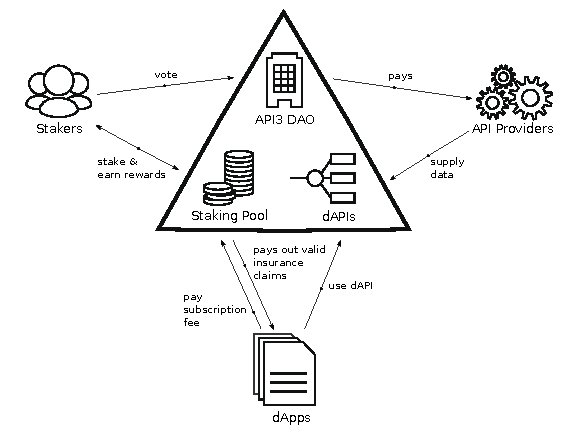
\includegraphics[width=0.9\textwidth]{fig/teaser/teaser}
	\caption{Overview of API3 mechanics.}
	\label{fig:teaser}
\end{figure}

API3 is a collaborative effort to build, manage and monetize dAPIs at scale.
To achieve this in a fully decentralized way, the incentives of the participants will be reconciled through the governance, security, and value capture utilities of the API3 token.
The project will have a completely open and direct governance model, where any API3 token holder will be able to stake to obtain direct voting privileges in the API3 DAO.
In addition, stakers will receive a portion of the dAPI revenue, inflationary staking rewards and any additional benefits that the DAO may decide on in the future.
The staked API3 tokens will back an on-chain insurance service as collateral to provide dAPI users with quantifiable and trustless security guarantees (see Figure~\ref{fig:teaser}).

One of the fundamental flaws of existing oracle solutions is attempting to establish and maintain a parasitic connection with the data sources, which cannot produce a sustainable ecosystem.
In contrast, we start off with the recognition that the API providers are the engine of this project.
Therefore, they will not be abstracted away, but rather be attributed and compensated so that their interests are fully aligned with the interests of the greater API3 ecosystem.
We have already witnessed API providers’ eagerness in incentivizing adoption of their services by decentralized applications through providing free testnet calls for their paid APIs~\cite{honeycomb.market} and offering cash prizes for hackathons~\cite{honeycomb-hackathon}.
Cultivating this cooperation further will be one of the main sources of strength of API3.

Decentralized oracle network solutions employ third-party oracles because it is often not feasible for the API providers to operate their own oracle nodes.
This positions third-party oracles as expensive middlemen and forms an additional attack surface.
To eliminate these problems and have the API providers engage in the ecosystem further, API3 data feeds will be composed of first-party oracles operated by the API providers.
This will be made possible by Airnode, a fully-serverless oracle node that is designed to require no know-how, maintenance, or upkeep from the API provider.
The resulting dAPIs will be cost-efficient and secure against attacks from an intermediate layer of third parties.

In the case of a malfunction, the dAPI user will be able to claim compensation up to a pre-negotiated amount from the staking pool.
Kleros~\cite{kleros:2019}, an on-chain dispute resolution protocol, will be used to decide if the claim is to be paid out based on the presented evidence.
This will incentivize stakers to actively participate in governance to ensure that dAPIs are being managed transparently and in a way that minimizes security risks.
Successful governance---generating revenue from dAPIs while avoiding mistakes that will result in paying out insurance claims---will be rewarded in API3 tokens, which will create a positive feedback loop that will continually improve governance.

Refer to Figure~\ref{fig:teaser} again for an overview of our solution.
dAPIs are networks of first-party oracles that provide traditional API services in a decentralized and blockchain-native way.
The API3 DAO builds, manages and monetizes dAPIs at scale.
Decentralized applications pay a subscription fee to gain access to a dAPI.
API3 token holders stake into a pool to receive rewards and voting rights at the DAO.
This staking pool is used as collateral for an on-chain insurance service that provides dAPI users with a quantifiable level of security.
API3 improves upon the existing oracle solutions in terms of decentralization, cost-efficiency, security, transparency and ecosystem growth potential.

%~~~~~~~~~~~~~~~~~~~~~~~~~~~~~~~~~~~~~~~~~~~~~~~~~~~~~~~~~~~~~~~~~~~
\section{API Connectivity Problem}
\label{sec:api-connectivity-problem}

An application programming interface (API) is a well-standardized and documented protocol that is used to communicate with a specific application to receive services from it.
These services may be in the form of receiving data or triggering an event.
Applications can communicate with each other through their APIs, allowing them to be integrated to build more complex applications.
Because of this, APIs are called the glue that holds the digital world together.

As a result of businesses using APIs to monetize their data and services, the concept of an API has transcended its initial meaning.
The term no longer refers to the technical implementation of an interface, but to a full-fledged product that includes the service it wraps~\cite{deloitte:2015}.
Global enterprises that provide APIs generate $25\%$ of their organizational revenue from APIs on average~\cite{mulesoft:2019}.
Companies such as Salesforce, Expedia and eBay have reported to generate the majority of their revenue through APIs~\cite{iyer:2015}, and we are at the cusp of fully API-centric business models~\cite{ibm:2016}.
Even entrenched industries such as banking are expected to be disrupted by this movement~\cite{capgemini:2019a}.

Integrating existing services to their applications through APIs has allowed developers to build increasingly complex and capable applications, which has led to the rise of giant Web services and mobile applications.
However, these APIs that businesses deliver their services through are not directly compatible with smart contracts due to technical reasons that will be described in Section~\ref{sec:oracle-problem-a-misnomer}, which has curbed the development of meaningful decentralized applications.
Therefore, the difficulty we are facing in building decentralized applications that can interact with the real world can presently be best described as the API connectivity problem.
Misinterpreting this problem will lead to a sub-optimal solution.

\subsection{Oracle problem: A source-agnostic misinterpretation}
\label{sec:oracle-problem-a-misnomer}

Decentralization defines Web 3.0, which is characterized by distributing computation and settling outcomes through predetermined consensus rules~\cite{nakamoto:2009}.
The business logic of a decentralized application is implemented as a smart contract~\cite{szabo:1994}, which runs on a blockchain-based smart contract platform~\cite{buterin:2014a}.
Decentralization allows participants to cooperate without requiring mutual trust or a trusted third-party, and thus provides robustness against attacks and censorship.

To enforce consensus rules, smart contract platform nodes have to verify that each contract invocation has resulted in the correct outcome by repeating the computation locally.
For this to be possible, smart contracts can only operate on information that is accessible to and agreed upon by all smart contract platform nodes.
In simpler terms, smart contracts can only operate on the information that is readily available in the blockchain, and cannot interact with the outside world directly.
This is widely known as the ``oracle problem'', referring to an idealized agent that can deliver an arbitrarily defined piece of truth to the blockchain.

The oracle problem is ill-posed, as even its name suggests an impossible solution.
An analogy would be to approach the problem of getting from Point~A to Point~B as the ``teleportation problem''.
Nevertheless, the first generation of solutions attempted to implement this literal oracle by posing a question and crowdsourcing its answer, which produces resolution times measurable in days and extreme gas costs due to the number of transactions that need to be made~\cite{augur:2019}, which is not ideal for use cases such as DeFi or prediction markets.
We must note that this approach is indeed suitable if the information to be delivered is subjective.
A good example would be the resolution of a judicial dispute~\cite{kleros:2019}.

The second generation solutions narrowed their scope to only cover factual information that can be accessed programmatically, and ended up with the ``interoperability problem''.
In these solutions, an oracle node that is integrated to two arbitrary systems (a blockchain and an API, two blockchains, etc.) acts as an automated intermediary between the two~\cite{ellis:2017,band,depedro:2017,tellor}.
Using multiple of these oracle nodes and settling on the outcome through predetermined consensus rules provides security guarantees that complement the underlying blockchain technology.
These solutions are faster and less expensive compared to crowdsourced oracles, and consequently are viable for more use cases, yet they suffer from being designed around an over-generalization of the problem at hand.

Interoperability solutions involve three parties: API providers, oracles, and data consumers~\cite{benligiray:2019}.
However, they fall into the pitfall of modeling their ecosystem as being solely composed of oracles and data consumers, while ignoring where the data originates from.
In other words, their models treat the oracle node as the mythical oracle that is the source of the truth.
Being blind to one-third of the problem in this way results in impractical solutions to be perceived as feasible.

The interoperability solution being source-agnostic results in the following consequences:
\begin{itemize}
    \item An intermediate layer of insecure and expensive third-party oracles, which could have been superseded by API provider-operated oracles;
    \item An ecosystem that nurtures rent-seeking middlemen, while excluding the actual sources of the data;
    \item Indiscriminate treatment of data received from different sources in a data feed.
\end{itemize}

Another pervasive issue with interoperability solutions is that since they are low-level protocols, they regard the interface as a technical component, or \textit{middleware}, rather than a complete product.
As a side effect, the governance of the interface gets left out-of-scope.
However, governance is hardly a trivial problem, because a decentralized interface requires independent and competing parties to cooperate.
The currently utilized solution is a trusted centralized entity to govern the interface, which is at odds with the main objective of decentralization.
The governing entity has full control over the output of an oracle network, which means a decentralized oracle network with centralized governance is a centralized oracle with extra steps.

\subsection{Decentralized APIs}
\label{sec:decentralized-apis}

The issues of the previous generation of interoperability solutions can only be solved by taking a new perspective: The problem at hand is in essence the problem of decentralized applications not being able to receive services from traditional API providers in a decentralized way.
Indeed, the primary use of interoperability solutions today is to deliver asset prices curated from centralized exchange APIs to DeFi applications, and emerging use cases such as prediction markets~\cite{omen} and parametric insurance~\cite{capgemini:2019b} all have similar requirements.
Therefore, further specifying the problem definition as such will allow us to arrive at the next generation of real-world interconnectivity solutions.

\begin{figure}
     \centering
     \begin{subfigure}{0.49\textwidth}
        \centering
         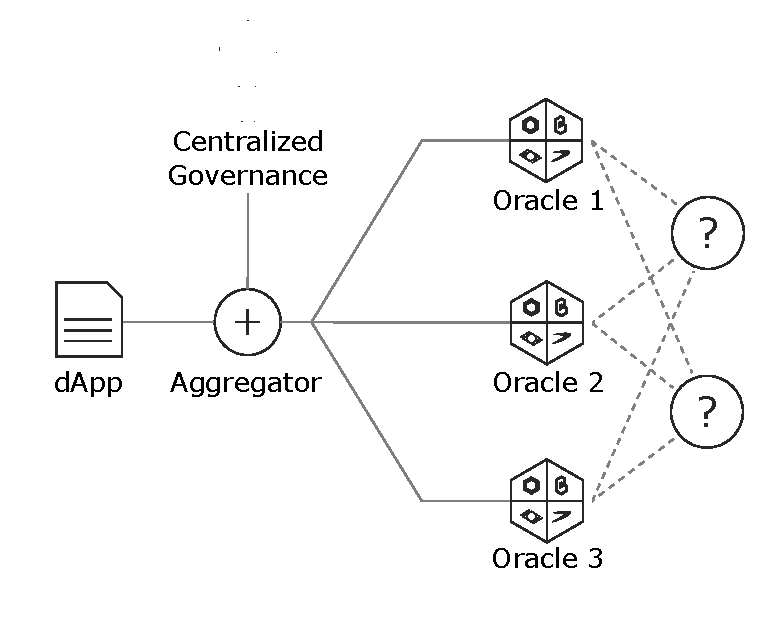
\includegraphics[height=5.7cm]{fig/solutions-comparison/solutions-comparison-a}
         \caption{Decentralized interoperability solution}
         \label{fig:solutions-comparison-3rd}
     \end{subfigure}
     \hfill
     \begin{subfigure}{0.49\textwidth}
        \centering
         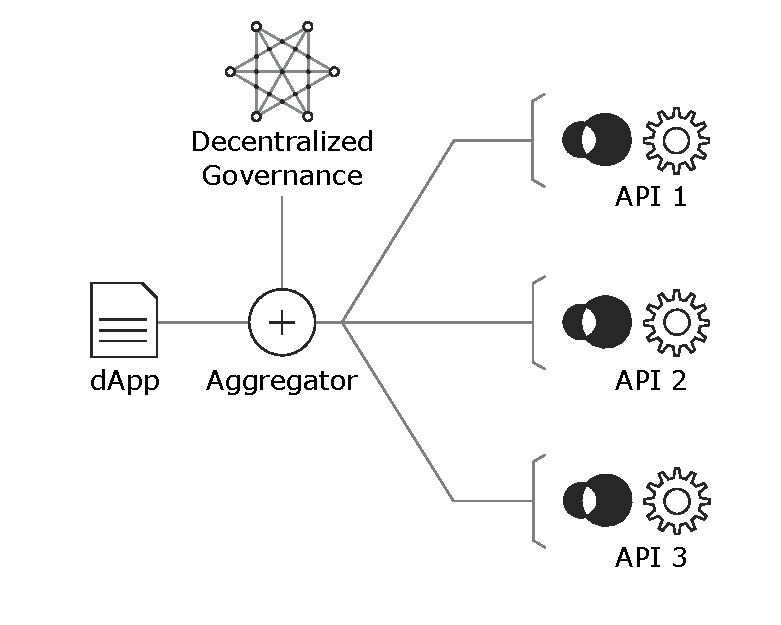
\includegraphics[height=5.7cm]{fig/solutions-comparison/solutions-comparison-b}
         \caption{Decentralized API (dAPI)}
         \label{fig:solutions-comparison-1st}
     \end{subfigure}
     \caption{Decentralized interoperability solutions employ third-party oracles that do not natively reveal their sources.
     dAPIs are composed of first-party oracles, meaning that API providers operate their own Airnodes.
     In addition, dAPIs are decentralized in how they are governed, resulting in end-to-end decentralization.}
    \label{fig:solutions-comparison}
\end{figure}

This new definition of the problem implies that decentralized applications require specific Web API services to be delivered to the blockchain and this to be done in a fully decentralized, cost-efficient and secure way.
Determining the requirements allows us to design a full product that satisfies them optimally:
Decentralized APIs, or dAPIs for short, are networks of API provider-operated first-party oracles that are governed in a decentralized way.
In contrast, decentralized interoperability solutions consist of an oracle network of third-party middlemen governed by a centralized entity, which is necessitated by their under-specified problem definition.
See Figure~\ref{fig:solutions-comparison} for a visual comparison.

%~~~~~~~~~~~~~~~~~~~~~~~~~~~~~~~~~~~~~~~~~~~~~~~~~~~~~~~~~~~~~~~~~~~
\section{Issues with Third-Party Oracles as Middlemen}
\label{sec:issues-with-third-party-oracles-as-middlemen}

Existing solutions envision an abstract problem where an arbitrary system needs to be able to interoperate with another arbitrary system through their technical interfaces in a very general sense.
This over-generality necessitates an ever-flexible interface that can only be supported by third-party oracles.
However, this solution is not optimal because the practical scope of the problem is far more constrained.
In most cases, the decentralized interoperability problem is actually the problem of receiving services from traditional API providers in a decentralized way.
This more limited definition of the problem allows for optimal solutions that do not require a third-party intermediate layer on the interface path.
Through the rest of this section, we will discuss the consequences of relying on middlemen as a part of an interoperability solution.

\subsection{Vulnerability}
\label{sec:vulnerability}

A decentralized oracle network uses an aggregation function to reduce the oracle reports into a single answer.
This function is essentially a consensus algorithm, and as all consensus algorithms, it is susceptible against a certain ratio of dishonest actors.
This means that a group of malicious oracles can collude to skew the outcome, and even control it completely.
In addition, a single actor can fabricate multiple oracle node operator identities—as well as build a sufficient track record of honest operation—to perform the same types of attacks entirely by themselves, which is known as a Sybil attack~\cite{douceur:2002}.

The most critical downside of having an additional layer of parties on the interface path is the formation of entirely new attack surfaces.
This means that each added layer of middlemen would be able to execute the collusion and Sybil attacks described above independently.
Then, in terms of security, the ultimate solution is the complete removal of the middlemen.

\subsection{Middleman tax}
\label{sec:middleman-tax}

\begin{figure}
    \centering
	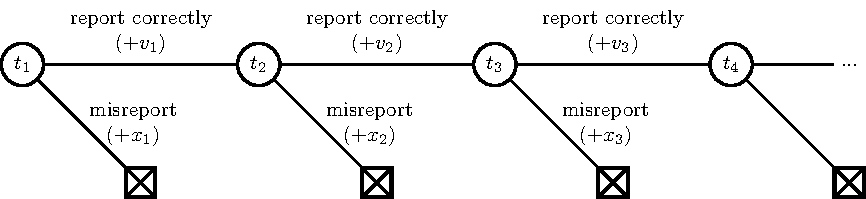
\includegraphics[width=\textwidth]{fig/decision-tree/decision-tree}
	\caption{A decision tree that describes the actions that an oracle can take and their outcomes.
	At a given transaction $t_i$, an oracle can report honestly and gain $v_i$ or misreport and gain $x_i$.
	A dishonest action results in the oracle no longer being used, i.e., an end to the game.}
	\label{fig:decision-tree}
\end{figure}

An oracle plays a game where they can report honestly or misreport (which includes denying service).
Reporting honestly has only an incremental payoff, but allows the oracle to continue playing the game.
On the other hand, misreporting has a one-time payoff proportional to the value secured by the contracts depending on the report, yet results in the game ending (see Figure~\ref{fig:decision-tree}).
Then, the maximum cumulative payoff the oracle can receive starting from transaction $t_i$ is

\begin{equation}
P \left[ i \right] = \max \left( x_i, v_i + P \left[ i + 1 \right] \right).
\end{equation}

A rational oracle will eventually misreport if the amount it can gain from an attack outweighs the potential gains it can make if it did not perform the attack.
That is, if the following holds for a given rational oracle, it will eventually misreport:

\begin{equation}
\exists i \in \mathbb{N},~ x_i > v_i + P \left[ i + 1 \right].
\end{equation}

This indicates that the potential benefit an oracle will gain from acting honestly must exceed the amount that can be gained from misreporting at all times to avoid any misreporting.
Although one can approximate $v$ with the amount paid to the oracle per-request and $x$ with the amount that is secured by the oracle’s response, this would underestimate the risk because there are additional factors that incline oracles towards misreporting, some of which are given below:

\begin{itemize}
    \item According to the time preference theory~\cite{frederick:2002}, the oracle node operator will value future rewards less (i.e., $v_i$ decays with increasing $i$).
    \item In practice, the oracle acting honestly does not guarantee the game to continue and this risk further lessens the value of future rewards.
    \item There may be additional benefits to performing an attack that are unaccounted for, e.g., opening a short position on an asset that will depreciate with the oracle solution’s failure.
\end{itemize}

Due to this uncertainty, one needs to overestimate the required $v_i$, i.e., overpay the oracle for it to not attack.

This model can be extended to decentralized oracle networks.
Since the oracle reports or their artifacts are recorded on-chain, it is trivial to implement a smart contract that will reward colluding oracles trustlessly.
This means that a third-party that is able to profit from an attack can employ oracles with the guarantee that they will be paid a deterministic amount if they collude.

At a high-level, an oracle’s job is essentially: (1) to listen for on-chain requests, (2) to make the respective off-chain API calls, and (3) to write the response back on-chain.
Therefore, a third-party oracle is fundamentally a middleman.
Although the service provided is as minimal as possible, these middlemen have to be paid proportionally to the amount being secured by the data feed due to the reasons described above, which is especially problematic for high-value use cases such as DeFi.
We call this phenomenon the ``middleman tax'', which can be eliminated completely by avoiding third-party oracles, resulting in very significant cost savings for users.

\subsection{Ineffective redundancy}
\label{sec:ineffective-redundancy}

\begin{figure}
    \centering
    \begin{subfigure}{0.513398876\textwidth}
         \centering
         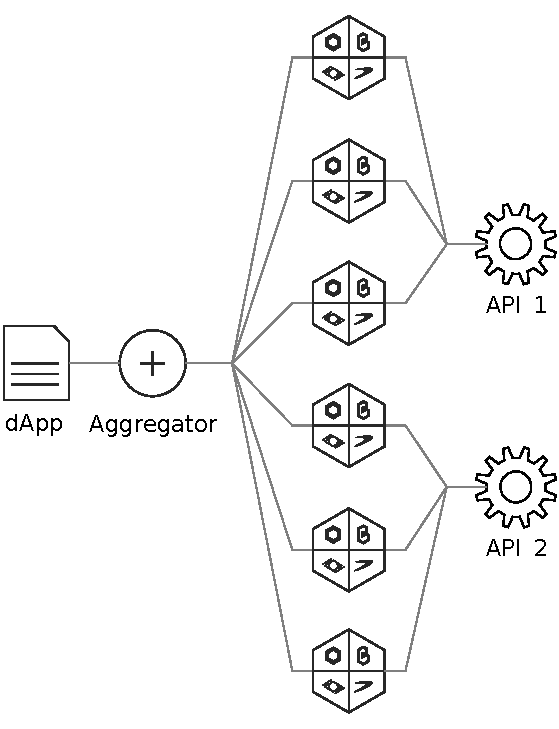
\includegraphics[height=8cm]{fig/oracle-level-decentralization/oracle-level-decentralization-a}
         \caption{Data feed composed of third-party oracles}
         \label{fig:oracle-level-decentralization-a}
     \end{subfigure}
     \hfill
     \begin{subfigure}{0.466601124\textwidth}
         \centering
         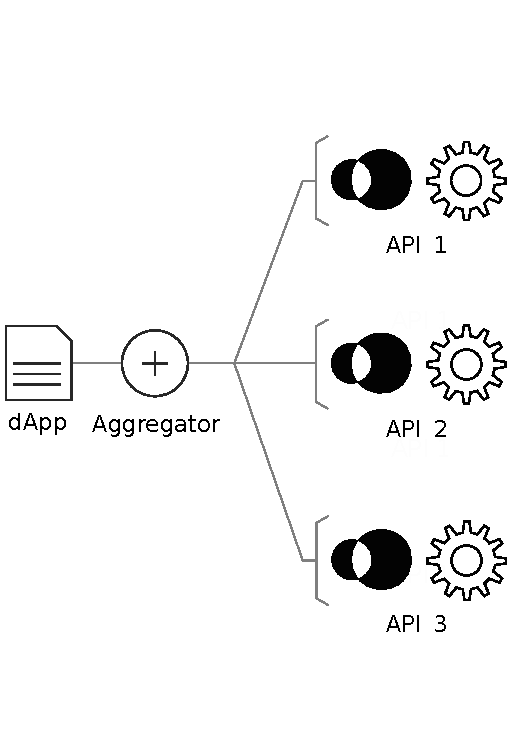
\includegraphics[height=8cm]{fig/oracle-level-decentralization/oracle-level-decentralization-b}
         \caption{Data feed composed of first-party oracles}
         \label{fig:oracle-level-decentralization-b}
     \end{subfigure}
	\caption{Using third-party oracles requires over-redundant decentralization at the oracle level, while first-party oracles provide a better degree of decentralization in a more secure and cost-efficient way.}
	\label{fig:oracle-level-decentralization}
\end{figure}

Data feeds depending on third-party oracles require over-redundancy at the oracle level (see Figure~\ref{fig:oracle-level-decentralization}).
This is because third-party oracles are far less trustworthy than API providers, the latter having a traditional off-chain business and respective reputation to maintain.
Typically, each API provider is served by 2--3 oracles in such a data feed.
Note that this decentralization does not provide additional security at the data source level, but only decreases the additional vulnerability caused by using third-party oracles.
Unfortunately, this results in the operation costs being multiplied on many levels.
For example, the data feed essentially employs all the technical personnel that operate the oracle nodes, and having more of these nodes means supporting more people.
Furthermore, using more oracles results in a direct increase in gas costs.
Specifically, oracle request--response gas costs increase linearly with the number of oracles, while the gas costs of aggregation functions that do combinational operations (e.g., median) increase superlinearly.

\subsection{Lack of transparency}
\label{sec:lack-of-transparency}

Decentralization at the API level and decentralization at the oracle level are independent of one another---the overall system is only as decentralized as the more centralized of the two, i.e., the weakest link.
However, the general public and even the users of decentralized oracle networks overlook this fact and confuse decentralization at the oracle level with the overall decentralization of the system.
This is primarily caused by a lack of transparency regarding the data sources used by the oracles~\cite{feeds.chain.link}, which disguises the fact that decentralization is severely bottlenecked at the data source (API) level.

Data feeds composed of third-party oracles appear more decentralized than they actually are.
In addition, when the data feeds are not transparent in the source of their data, developers cannot appraise data feed integrity and have to trust the governing entity.
However, there is no immediate incentive for the governing entity to choose quality over lower prices and convenience if the data sources are not transparent, which may result in the outcome commonly referred to as ``garbage in, garbage out''.

Interestingly, what is a favorable tactic for the governing entity---namely, obscuring the data source---is very much necessary for the third-party oracle.
Most API terms of service prohibit the resale or unauthorized distribution of the API data, which positions an oracle node operator serving such APIs to be in breach of those terms and susceptible to broad sources of legal liability including claims by the API provider~\cite{data-licensing}.
This issue is exacerbated by the API call times, responses, and payments all being recorded on a public blockchain.
This not only puts individual node operators at litigation risk, but also creates a systemic risk for the whole oracle network, as coordinated legal action at scale would put existing third-party oracles out of operation immediately and discourage new ones from joining.

Note that although lack of transparency and abstraction of data sources is the norm, it is not at  all a necessity.
Especially when the API provider and ecosystem incentives are aligned, it is perfectly possible for oracles to serve API data to users with the express consent of the API provider, allowing the oracles to disclose their data sources to their users~\cite{honeycomb.market}.
It is in the interest of the API providers to do this, as it increases on-chain demand for their data.

%~~~~~~~~~~~~~~~~~~~~~~~~~~~~~~~~~~~~~~~~~~~~~~~~~~~~~~~~~~~~~~~~~~~
\section{Airnode: A Node Designed for First-Party Oracles}
\label{sec:airnode-a-node-designed-for-first-party-oracles}

First-party oracles are integral to the API3 solution.
This means each API is served by an oracle that is operated by the entity that owns the API, rather than a third-party.
In this section, we will discuss the benefits of using first-party oracles, why it is not feasible for API providers to operate their own oracles with current available solutions, and how we aim to solve this problem with Airnode.

\subsection{Benefits of disintermediation}
\label{sec:benefits-of-disintermediation}

There is a simple solution to all problems discussed in Section~\ref{sec:issues-with-third-party-oracles-as-middlemen}: First-party oracles; that is, oracles operated by the API providers themselves.
API providers operating their own oracles means they would be signing their responses with their private keys at the smart contract platform protocol-level, which is the best proof that the data is not tampered with.
Moreover, first-party oracles are private by default, as a third party cannot observe the raw data from the API being processed, which allows them to be used in a wider variety of use cases natively.

A data feed composed of first-party oracles would be more cost-efficient compared to one employing middlemen, as one needs to pay middlemen both for their services and to incentivize them against attacking the data feed (referred to as the middleman tax in Section~\ref{sec:middleman-tax}).
In addition, a data feed composed of first-party oracles will need fewer oracles, as it would not need over-redundant decentralization at the oracle level to protect against attacks from third-parties.
Assuming that each API is typically served by at least two third-party oracles, data feeds powered by first-party oracles would be at least $50\%$ more efficient in terms of gas costs, by a conservative estimate.

First-party oracles also provide much needed transparency in terms of the data source and the degree of decentralization.
Since each API provider will operate an oracle---which will be visible on-chain---the number of oracles serving a data feed will accurately represent how decentralized it is, as there is a one-to-one mapping between oracle and data source.
Furthermore, the API providers would publish their on-chain identities through off-chain channels, which would allow the users to verify whose data they are consuming at a given time.

Finally, having the API providers operate the oracles solves the legal issues mentioned in Section~\ref{sec:lack-of-transparency}, as the API services no longer need to be licensed to a third party and the API providers receive the entire revenue.
Furthermore, this solves the rent-seeking third-party oracles problem, and allows the funds to be redirected to the group that is doing the heavy lifting, the API providers.
Incentivizing API providers aligns their financial interests with the ones of the API3 ecosystem, resulting in a strong mutual bond between the two.

\subsubsection{Off-chain signing of data}
\label{sec:off-chain-signing-of-data}

There is a hybrid solution that still depends on third-party oracles, yet does not let them tamper with the data.
In this scheme, the API provider signs their data with their private key off-chain and serves it over a regular API endpoint.
Third-party oracles call this endpoint to get the signed data and post it to the chain.
The authenticity of the data---that it is not tampered with by the third party oracles---can then be verified on-chain using the public key of the API provider~\cite{open-price-feed}.

Although it eliminates the risk of data tampering at the oracle level, this solution is essentially a half-measure.
By depending on third-party oracles, it continues suffering from the ecosystem issues caused by depending on third-party oracles, and, in addition, requires modifications at the API-side to implement off-chain signing.
This results in a severely limited API selection even compared to the regular third-party oracle based solutions, and restricts the ecosystem growth potential of the solution to the application-scale.

\subsection{Barriers to API providers operating oracles}
\label{sec:barriers-to-api-providers-operating-oracles}

During our work on Honeycomb API Marketplace~\cite{benligiray:2019} in the past two years, we communicated with API providers extensively and observed the following barriers to oracle onboarding and operation:

\begin{enumerate}
    \item Traditional API providers are typically not more familiar with blockchain technologies than the general public.
    This applies even for the ones that curate cryptocurrency market data---as their main operation is collecting data from exchange APIs, processing them, and serving the result through their own APIs---which does not require any blockchain-specific know-how.
    Therefore, they typically cannot readily operate an oracle node with in-house resources.
    \item There is no job market for oracle node operators.
    Even if some API providers were to obtain the specific know-how needed by hiring the few node operators that are available, this would not be a scalable solution.
    \item Operating an oracle node consumes a lot of resources in the form of man-hours and infrastructure costs.
    Unless one is guaranteed significant subsidies or future profits, operating an oracle node is financially infeasible.
    \item Operating an oracle node requires the API provider to transact with cryptocurrencies.
    Specifically, they must pay for gas costs in the native currency (e.g., ETH) and receive payments in one or more cryptocurrencies.
    This disqualifies the vast majority of API providers due to compliance, legal and accounting reasons.
    In addition, any scheme that requires API providers to stake funds is categorically rejected for similar financial risk-related reasons.
\end{enumerate}

\subsection{Airnode features}
\label{sec:airnode-features}

\begin{figure}
    \centering
	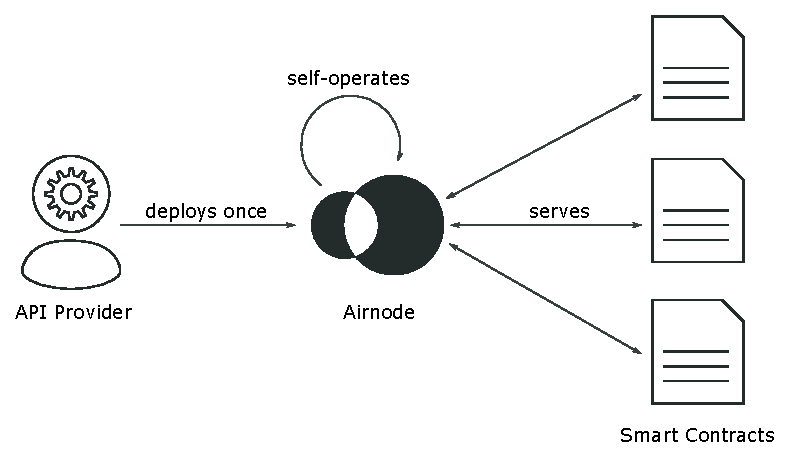
\includegraphics[width=0.8\textwidth]{fig/airnode/airnode}
	\caption{Airnode is designed to be deployed once by the API provider, then not require any further maintenance.}
	\label{fig:airnode}
\end{figure}

Airnode is a fully-serverless oracle node that is designed specifically for API providers to operate their own oracles (see Figure~\ref{fig:airnode}).
It addresses all of the oracle node-related problems in Section~\ref{sec:barriers-to-api-providers-operating-oracles}:

\begin{enumerate}
    \item It does not require any specific know-how to operate.
    In fact, it is difficult to even speak of an operation, as Airnode is designed to be completely \textit{set and forget}.
    \item It does not require any day-to-day maintenance such as updating the operating system or monitoring the node for uptime owing to existing fully managed serverless technology.
    It is designed to be stateless, which makes it extremely resilient against any problem that can cause permanent downtime and require node operator intervention.
    \item It is built on services priced on-demand, meaning that the node operator is charged only as much as their node is used.
    This allows any API provider to run an oracle for free and start paying only after they start generating revenue.
    \item It does not require the node operator to handle cryptocurrency at all.
    Its protocol is designed in a way that the requester covers all gas costs.
\end{enumerate}

One way to see Airnode is as a lightweight wrapper around a Web API that allows it to communicate with smart contract platforms with no overhead or payment token friction.
Regarding the level of involvement required from the API provider, using Airnode can be likened to utilizing an API gateway that makes an API accessible over the Web, rather than operating a blockchain node as a side-business.
In fact, our aim is for Airnode to become as ubiquitous and mundane for APIs as using an API gateway, which will make a vast variety of first-party oracles available to API3.

API providers invest significant resources to build a highly available infrastructure.
Then, it is important for the oracle node implementation to not contain single points of failure that may cause downtime.
Existing solutions using third-party oracles depend on over-redundancy at the oracle level to cover for this, which results in excessive costs as mentioned in Section~\ref{sec:ineffective-redundancy}.
API3 envisions each API to only be served by its first-party oracle, which means the redundancy has to be implemented at the level of the individual Airnode.
The node being fully-serverless enables this to be done easily across different availability zones of a single cloud provider, or even across multiple cloud providers.
It should also be mentioned that it will be possible to containerize Airnode and operate it on-premises, yet using the serverless version will be recommended for almost all use cases.

Airnode is developed by the founding members of API3 and is now open-sourced\footnote{\url{https://github.com/api3dao/airnode}}.
The software is feature-complete for the protocol described in Section~\ref{sec:airnode-protocol}, and further development will be funded by API3 in the form of grants.

\subsection{Airnode protocol}
\label{sec:airnode-protocol}

Similar to how we prefer the better specified API connectivity problem over the oracle problem, we believe that an oracle node should be designed to interface APIs to smart contract platforms very well, rather than as a sandbox that can purportedly be used for any purpose imaginable.
Based on this philosophy, the Airnode protocol is designed to follow the self-emergent patterns used by APIs to achieve as transparent and frictionless of an API--smart contract platform interface as possible.

The first and the most commonly used API style follows the request--response pattern, where the user makes a request with parameters and the API responds as soon as possible.
This will be the first pattern that Airnode will support, as it is easy to standardize and integrate with existing APIs that follow the same pattern.
An example use case of this scheme would be requesting the result of a specific match to be delivered, which can be used to resolve the respective prediction market.
In addition, Airnode is planned to support the publish--subscribe pattern, where the user requests the oracle to call back a specific method when parametrized conditions are met.
For example, a decentralized exchange may request the oracle to trigger a liquidation event for a user in a leveraged position when ETH price drops below \$400.
Either of these patterns can be used to implement the live data feeds that DeFi applications use today~\cite{liu:2020}, but they can also support a much larger variety of use cases in the form of dAPIs.

As mentioned in Section~\ref{sec:airnode-features}, the Airnode protocol is designed in a way that the requester assumes all gas costs, even including the request fulfillment transactions.
This is achieved by each Airnode having a separate wallet for each requester, similar to how cryptocurrency exchanges automatically designate wallets for users to deposit funds to.
The requester funds this wallet with the native currency (e.g., ETH), either in a lump sum or through per-request microtransactions.
The funds in this wallet are used to fulfill all of the following requests made by the requester.
This scheme has significant advantages:

\begin{itemize}
    \item The volatility in gas costs and payment token prices (e.g., LINK) makes it virtually impossible for oracles to set profitable yet competitive prices.
    Calculating prices dynamically on-chain requires multiple data feeds and adds a significant gas overhead per-request.
    With the Airnode protocol, the API providers do not have to concern themselves with gas costs, and can use pricing schemes such as \$0.1 per call or \$100 per month, which is similar to typical API pricing models.
    \item As mentioned in Section~\ref{sec:barriers-to-api-providers-operating-oracles}, it is not reasonable to expect API providers to be able to convert fiat into cryptocurrency and fund their node wallets as a part of their day-to-day operations.
    In this scheme, the node operator never has to think about their node wallet balance.
    \item As seen in a recent attack performed on Chainlink data feeds~\cite{chainlink-gastoken}, oracle nodes that use a common wallet to fulfill requests are susceptible to attackers spamming requests to drain their wallets.
    The solution to this is for the node operators to maintain a whitelist of trusted addresses that they will accept requests from.
    In addition to the difficulty of determining which contracts are supposed to be trusted in this context, this renders any kind of public listing service practically infeasible.
    This is a critical issue, as it stops the little independent ecosystem growth there is dead in its tracks.
    Airnode is not susceptible to this type of an attack, as a requester's designated wallet is only used to fulfill requests from the said requester, and cannot be drained by others.
    \item Traditional oracle nodes have to fulfill all requests with very high gas prices, as they cannot tolerate their transaction queue being blocked by a single transaction made with a low gas price.
    With the Airnode protocol, this is no longer a concern, as each requester will have a separate transaction queue.
    Then, requesters whose requests are not time-critical would be able to provide the fulfillment gas price as a request parameter and enjoy service at a much lower gas cost.
    This scheme can be expected to synergize with EIP1559~\cite{eip1559}.
\end{itemize}

Finally, let us briefly mention how the Airnode protocol approaches monetization.
It is common for a project-specific token to be worked into the core of the protocol in an attempt to ensure that the said token is needed.
However, this induces an enormous gas price overhead, severely restricts alternative monetization options and creates overall friction.
For these reasons, the Airnode protocol purposefully avoids using such a token.
Instead, the node operator is allowed to associate custom authorizer contracts to their oracle endpoints, which essentially decide if a requester should be responded to based on any criteria that can be implemented on-chain.
The authorizer contracts can be used to enforce whitelists, blacklists, monthly subscription payments or per-call fees.
This scheme is both very flexible, and is implemented in a way that does not add any gas cost overheads.
Although dAPI monetization is a completely independent matter, the flexibility that Airnode provides will carry over, e.g., it will be possible to implement a dAPI where the users assume all gas costs, which is not possible with the existing oracle solutions.

\subsection{API integrations}
\label{sec:api-integrations}

There is a chicken-and-egg problem when it comes to integrating APIs to oracles.
If there is no existing demand for an API in an oracle ecosystem, nobody is incentivized to do the integration.
If the API is not available due to a lack of integration, nobody develops applications that will create the demand.
This was identified as a key friction point for the Chainlink ecosystem, and Honeycomb API Marketplace was proposed as a solution~\cite{benligiray:2019}, which has been operational for over a year~\cite{honeycomb.market}.
Honeycomb has integrated a large number of premium APIs to Chainlink oracles, and as a result, this marketplace serves an API variety that is unmatched in any oracle ecosystem.

Honeycomb uses a universal external adapter and a novel method to integrate APIs to Chainlink oracles in a declarative way, without requiring any code to be written.
This method is superior to developing an external adapter for each API operation~\cite{external-adapters} in that its integrations are faster, less error-prone, and can be done by non-experts.
Using these proprietary tools, Honeycomb was able to integrate hundreds of unique API operations in a few months, which dwarfs the closest competition by an order of magnitude.

For API3 to reach its full potential, it will need hundreds, if not thousands of first-party oracles so that it can easily set up new dAPIs or recompose existing ones.
This can only be achieved if APIs can be integrated to Airnode in an even more scalable way.
To this end, an improved version of the proprietary integration tools described above will be open sourced for Airnode.
Borrowing from the OpenAPI Specification format~\cite{oas}, Oracle Integration Specifications (OIS) define the operations of an API, the endpoints of an oracle, and how the two map to each other.
An Airnode user will be able to serve an API over their oracle simply by providing its OIS to their node.
Integrations made in this standardized format will be very easy to collect, version and distribute.

OIS is a JSON file, primarily designed to describe the integration specifications for Airnode to use.
This means that it does not aim to be human-readable first and creating it manually to specify an integration would be difficult.
This problem will be solved by ChainAPI, an integration platform that will allow users to generate OIS for their APIs through an easy-to-use graphical interface.
This will be accompanied by other quality of life improvements for Airnode users, such as a node dashboard and a marketplace to list their endpoints.
As a result, API3 will have a wide selection of first-party oracles to compose dAPIs from and ecosystem growth will no longer be bottlenecked by integration capacity.

%~~~~~~~~~~~~~~~~~~~~~~~~~~~~~~~~~~~~~~~~~~~~~~~~~~~~~~~~~~~~~~~~~~~
\section{Decentralizing Governance through Tokenomics}
\label{sec:decentralizing-governance-through-tokenomics}

A single point of failure is a critical component of a system where, if failure occurs, there is no redundancy to compensate, causing the entire system to fail.
Centralization produces single points of failure and decentralization aims to eliminate them.
Blockchain-based applications implicitly claim decentralization, yet the majority are still centralized in some aspects, notably governance~\cite{Walch:2019}.
In this section, we will discuss the problems arising from centralized governance and how API3 will solve these by way of a decentralized autonomous organization (DAO)~\cite{buterin:2014b} with well-designed tokenomics.

\subsection{Centralized oracle network governance}
\label{sec:centralized-oracle-network-governance}

If a decentralized oracle network is configurable by a centralized entity, its governance is centralized.
This may cause governance mistakes to go unnoticed, which may result in the data feeds misreporting even when the underlying APIs and oracles are functioning correctly.
For example, the Chainlink~\cite{ellis:2017} silver price data feed reported the gold price for a period of time due to a governance mistake caused by human error~\cite{chainlink-fatfinger}.
Synthetix~\cite{synthetix:2020}, a decentralized exchange for derivatives, was using this data feed at the time, resulting in some of their users exploiting the error for profit~\cite{synthetix-fatfinger}.
Due to its inherent opaqueness, centralized governance allows the usage of substandard practices, which inevitably result in such consequences.
However, the more glaring issue that this event has demonstrated is that a centralized governing entity can trivially use their authority to maliciously misreport.

The governing entity has the authority to recompose a data feed, which means switching oracles and their respective data sources in and out.
This is required for long term maintenance of the data feed, yet it exposes the data feed user to a variety of abuses and attacks by the governing entity.
Then, the users either have to trust a centralized governing entity, or the governance of the data feed has to be decentralized with incentives that favor security.

In the case where the data feed user feels they can trust a central governing entity completely, using a decentralized oracle network is irrational and the user would be better served by using a centralized oracle operated by the governing entity.
Firstly, as discussed in Section~\ref{sec:vulnerability}, this centralized oracle would not have third-party oracles as an attack surface and would thus be more secure.
Furthermore, a centralized oracle would provide much better performance in terms of availability due to the difficulty in coordinating a large number of oracle node operators, which sometimes causes data feed-level outages~\cite{chainlink-outage}.
Finally, the operating cost of such a centralized oracle would be far lower than an oracle network.
Therefore, we contend there is no circumstance where centralized governance of oracle networks can be justified.

\subsection{Management of funds}
\label{sec:management-of-funds}

Initial coin offerings (ICOs) have been a popular fundraising method for blockchain projects, which typically involve the development team to be fully trusted with the development funds.
Although this is sensible on the surface, it gets challenged when the token price increases speculatively, which results in the development team gaining control of a much larger amount than what the investors trusted them with in the first place.
Since it is well established that centralized governance is strongly associated with corruption~\cite{fisman:2002}, we can say that this has the potential to lead to deceitful outcomes ranging from exit scams to development funds being misused in order to manipulate the token price further, resulting in unsustainable growth.
This risk is heightened with a lack of budget transparency, which unfortunately is the norm.
In addition to the technical development fund, some projects have an additional ecosystem development fund.
It is even more difficult to justify giving the control of these funds to the development team, as they are only a part of the ecosystem and do not necessarily represent it and share its interests as a whole.

DAICOs (an amalgamation of the terms DAO and ICO) have been proposed as a solution to these problems, which involves a DAO of investors to allocate a stipend to the development team, which can be regulated and even completely cut off by the DAO~\cite{buterin:2018}.
A more flexible approach that is being employed by DAOs successfully today is to conduct the entire development through grants~\cite{dxdao:2019}.
In this scheme, the DAO does not have a development team, but rather jobs to do, and it contracts third parties to work on them on a case-by-case basis.
This typically results in honest and efficient allocation of development and ecosystem funds at actual market rates.

\subsection{API3 DAO}
\label{sec:api3-dao}

To decentralize the governance of both dAPIs and the project as a whole, API3 will be governed by a DAO.
The governance will be entirely decentralized and open, meaning that all stakeholders will be able to participate in the governance of the project directly.
This will be achieved through the API3 token, which will grant voting power in the API3 DAO through the mechanics described in Section~\ref{sec:api3-tokenomics}.

The core governance structure will be built on DAOstack, a framework for building decentralized autonomous organizations~\cite{daostack:2018}.
The DAO will vote on high-level parameters regarding mechanics such as staking incentives and collateralization.
Additionally, the DAO will give out grants from the DAO bank and by consequence decide on the general direction of the project.
More granular tasks will be conducted through hierarchical team structures for scalable governance.

The expected workflow is for people to form off-chain teams and apply for grants to execute one-time projects or continuous operations that will benefit API3.
The team makes the grant application with a multisig that has the team members assigned as users (e.g., Gnosis Safe~\cite{gnosis}), and the DAO grants the funds to the multisig if the grant proposal is accepted.
Furthermore, the DAO may authorize the team multisig to make specific transactions depending on the assigned task, e.g., setting dAPI subscription fees for individual users.
Note that team members may have to disclose their real identities for projects with critical responsibilities and large budgets to verify their credentials and avoid potential Sybil attacks.

Examples of technical grant subjects can be listed as follows:
\begin{itemize}
    \item Technical development of Airnode, dAPI contracts, API3 DAO contracts
    \item Frontend development for API3 (staking, insurance, etc.)
    \item Development of API3 ecosystem projects
    \item Integration of new APIs, dAPI users, smart contract platforms
    \item Statistical and qualitative risk assessment for specific APIs and dAPIs
    \item Managing dAPIs
    \item Developer outreach through articles, tutorials, videos
    \item Technical and security audits
    \item Setting up bug bounty programs, hackathons, etc.
\end{itemize}

There is also an abundance of non-technical tasks that will be carried out through grants:
\begin{itemize}
    \item Business development to find new API providers, dAPI users
    \item Subscription and insurance pricing for specific dAPI users
    \item Operational and financial audits
    \item Payment processing
    \item UI/UX design
    \item Marketing
    \item Legal counsel
\end{itemize}

\begin{figure}[t]
    \centering
	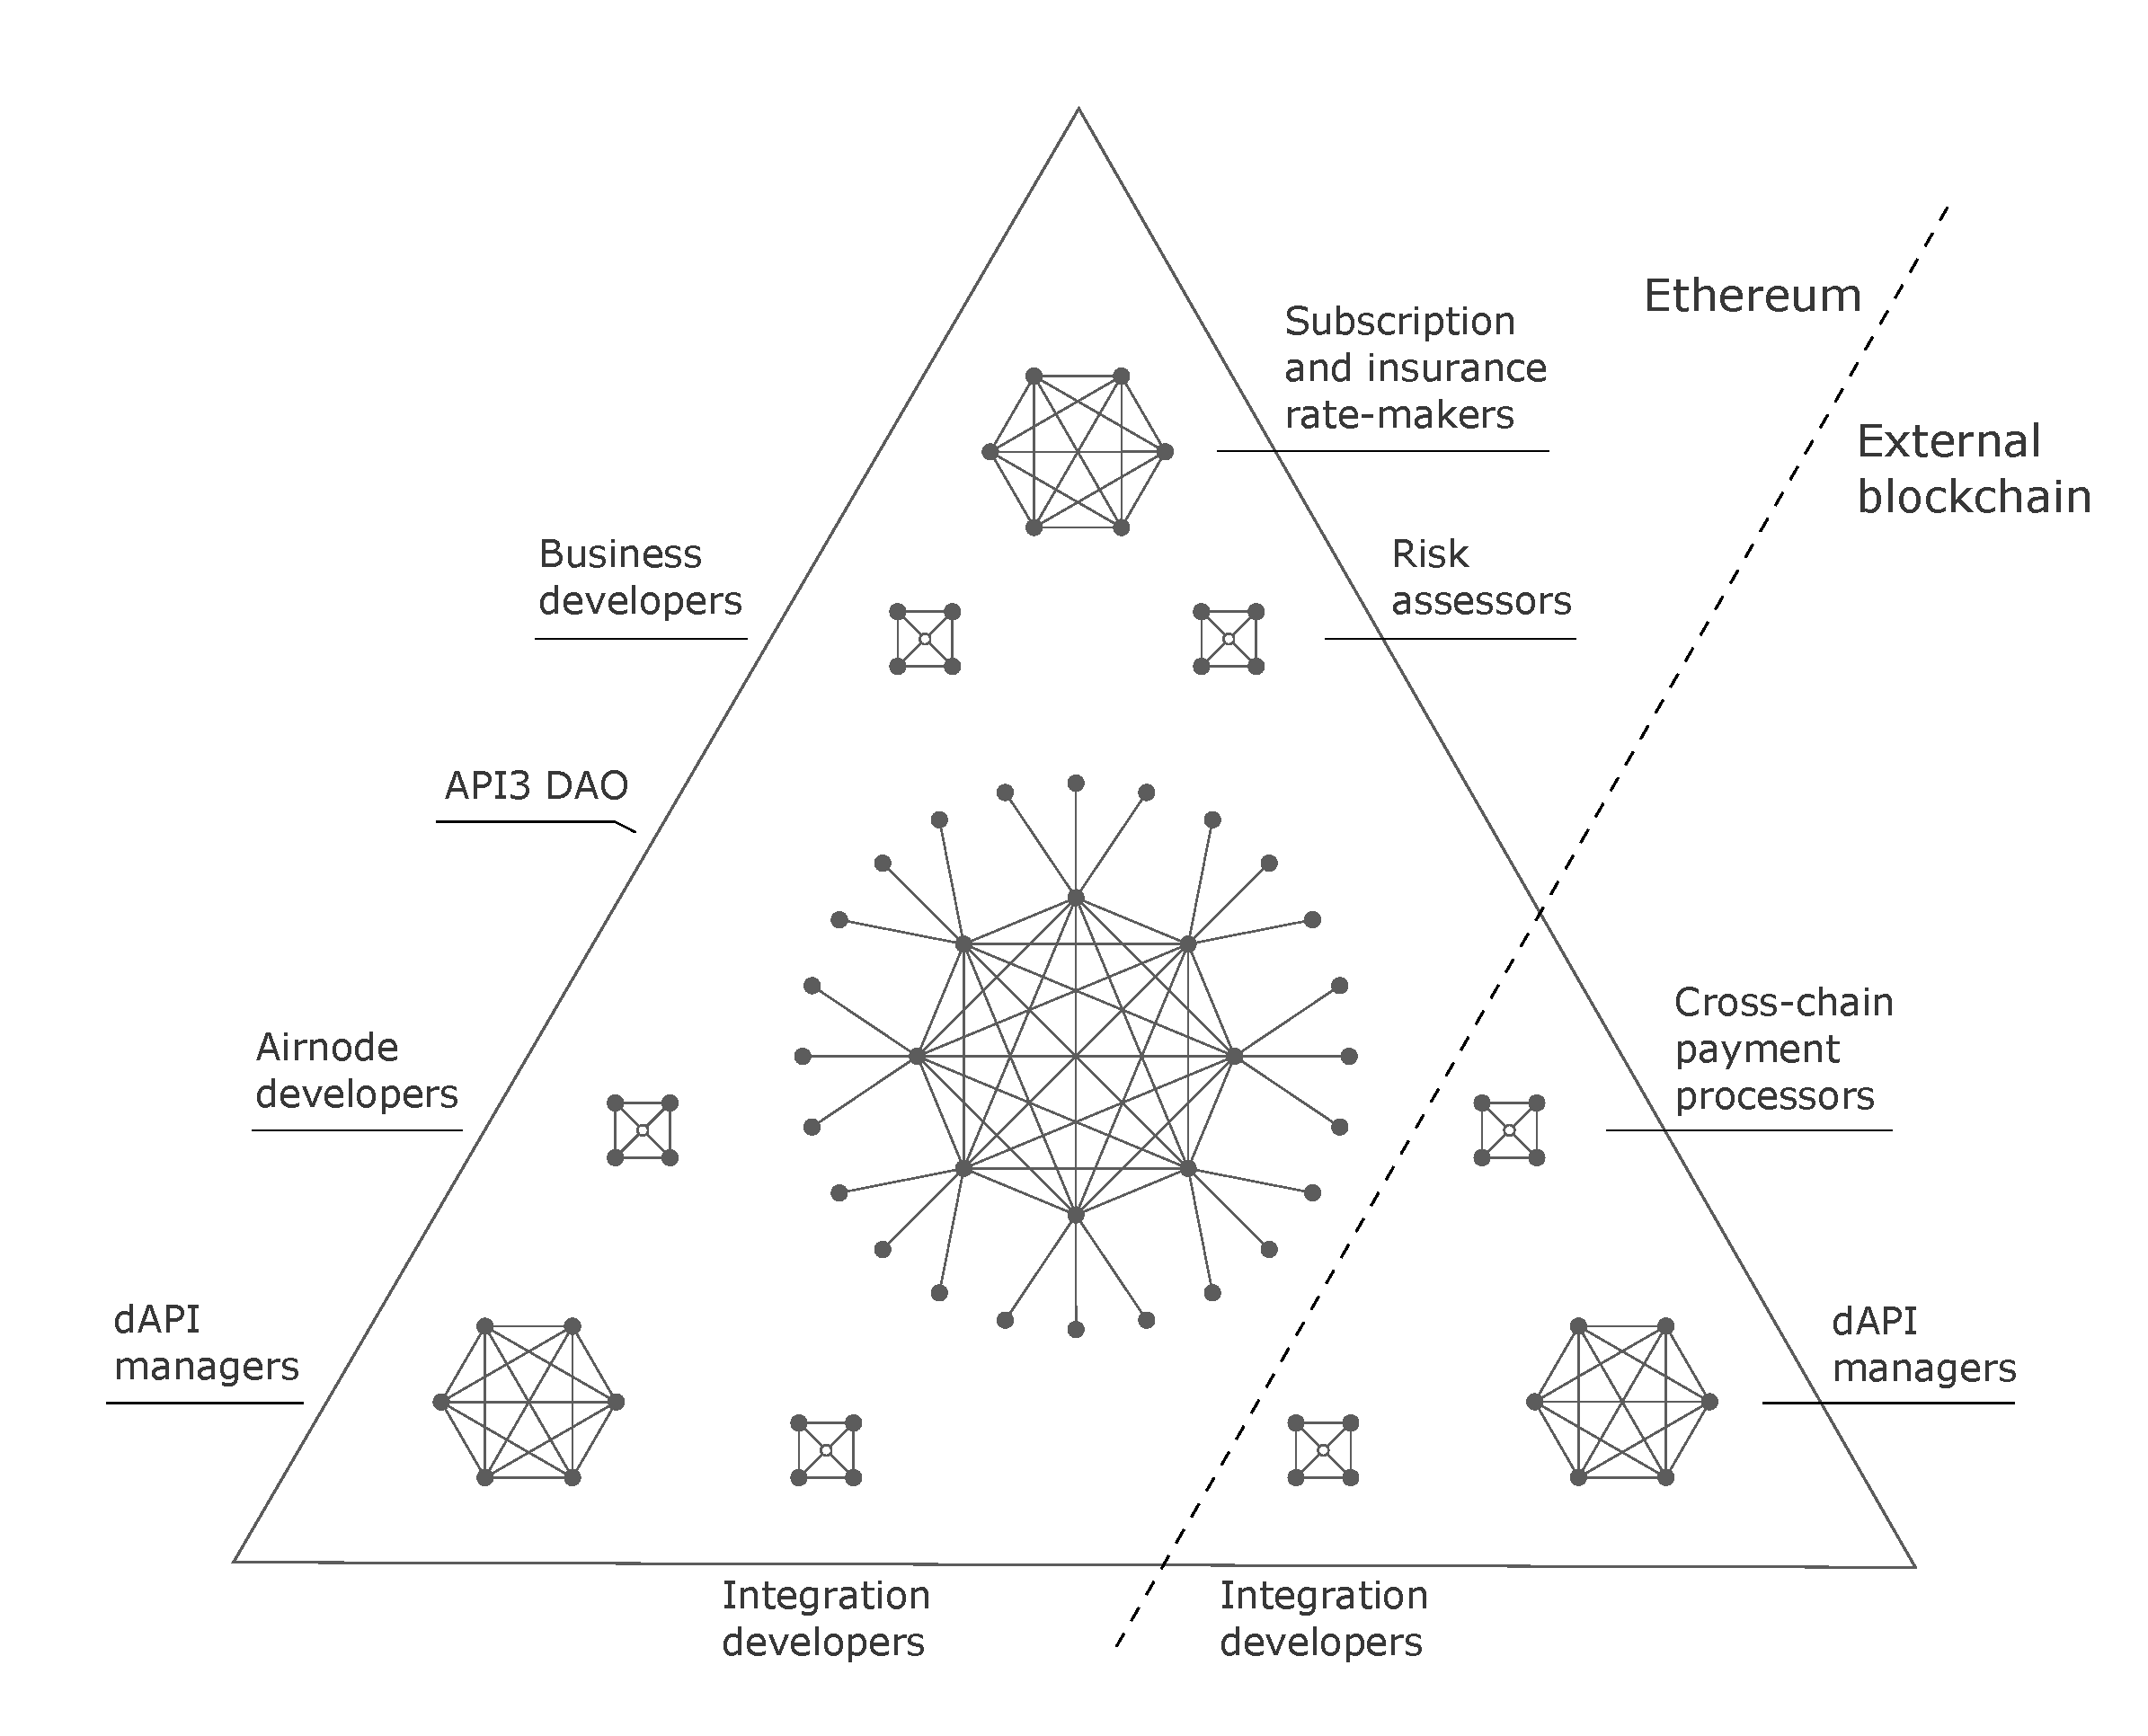
\includegraphics[width=\textwidth]{fig/dao/dao}
	\caption{An example hierarchical governance structure, composed of the main DAO, subDAOs and teams distributed across chains.
	The main DAO governs by selectively allocating funds and delegating authority.
	When a task reaches a scale that can no longer be fulfilled by a team, it is assigned to a subDAO.}
	\label{fig:dao}
\end{figure}

This team-based governance scheme is scalable in terms of gas costs, as it requires fewer proposals to be voted on at the DAO level.
It is also more scalable in practical terms, as it does not require the constant attention of all governing parties to a wide variety of minute details.
Furthermore, it allows critical operations such as dAPI management to be executed swiftly and based on expert opinion.
As API3 operations scale up, this governance hierarchy may demand additional layers, which implies subDAOs (see Figure~\ref{fig:dao}).

The DAO must follow two principles for this scheme to be effective.
Firstly, to limit the amount of damage a malicious or incompetent team may cause, the authority that the team has must be constrained to a bare minimum, which is also known as the ``principle of least privilege''.
For example, a dAPI management team should never be able to completely recompose a dAPI that is under use, but should only be able to switch individual oracles in and out with a long enough cool-down period to ensure that their authority cannot be abused to a significant degree.
Similarly, milestones and deliverables should be utilized to grant teams only the funds they need to carry out the specific responsibilities they have at the time.
The second principle is transparency.
For the DAO to be able to assess its performance, the team must report to the DAO in great detail.
These reports will have the additional benefit of providing accountability and allow the dAPI users and the general public to be able to audit the operations of API3 at all times.

\subsection{dAPI monetization and API provider compensation}
\label{sec:dapi-monetization-and-api-provider-compensation}

API subscription fees are commonly paid monthly or annually, as this scheme suits both API providers and their clients.
API3 will aim to follow the same scheme for dAPIs.
To gain access to a dAPI, the user will pay a recurring subscription fee, which may either be fixed or customized for the user based on the specific use case.
These prices will be determined by the respective team, and will include the premium if the user wants to receive the insurance service described in Section~\ref{sec:quantifiable-security-through-insurance}.
The payment will be able to be made in any cryptocurrency, which will be received by the DAO in API3 tokens through a liquidity pool-based decentralized exchange.

API providers will be compensated periodically at fixed rates, which will fit their existing pricing models.
This will be done using stablecoins wherever possible, yet as mentioned in Section~\ref{sec:barriers-to-api-providers-operating-oracles}, some API providers categorically reject handling cryptocurrency as payment.
In such cases, the DAO will provide a grant that will be paid out in return of the proof that the API provider is compensated in fiat by the grantee.

\subsection{Cross-platform dAPIs}
\label{sec:cross-platform-dapis}

API3 will utilize xDai~\cite{xdai:2019} as a second layer scaling solution, and thus working in a cross-platform way will be an ordinary part of its operations.
The same workflow that will be developed to bridge xDai to Ethereum will be used to bridge to other smart contract platforms, allowing API3 to serve cross-platform dAPIs.
These cross-platform integrations will be implemented and maintained through grants, which will be given to teams partly composed of parties from the respective smart contract platform ecosystems.

We have described a scheme for compensating API providers in fiat currency in Section~\ref{sec:dapi-monetization-and-api-provider-compensation}.
Regarding cross-platform dAPI subscription fees, we need the API3 DAO to be compensated across smart contract platforms, which is a similar problem.
Therefore, we will use an analog of the same solution, where a grantee will pay the API3 DAO in return for being authorized to receive payments on its behalf on another smart contract platform.
For example, if the DAO needs to be paid 100 API3 tokens as the subscription fee, the grantee will pay 90 API3 tokens to the DAO, which will result in the understanding that the grantee is authorized to receive the 100 API3 tokens-worth of payment on another chain.
This process will be formalized as required.

By implementing the data bridge and the payment channel, API3 will be able to serve other smart contract platforms without requiring them to interact with Ethereum or handle API3 tokens.
Note that Ethereum will be used as the dispute resolution layer for the insurance service described in Section~\ref{sec:quantifiable-security-through-insurance} until a cross-platform alternative emerges.

\subsection{API3 tokenomics}
\label{sec:api3-tokenomics}

Decentralized governance requires well-balanced incentive mechanisms that accurately model both positive and negative outcomes.
In other words, the governing entities should be rewarded for good results and penalized for bad ones.
The API3 token is designed to facilitate this through three main utilities:

\begin{enumerate}
    \item Staking: Grants dAPI revenue and inflationary rewards.
    \item Collateral: Backs insurance services that protect users from damages caused by dAPI malfunctions.
    \item Governance: Grants direct representation in the API3 DAO.
\end{enumerate}

The staking utility provides a financial incentive for participating in API3 and contributing to increase its revenue.
The collateral utility has the participants share API3’s operational risk and incentivizes them to minimize it.
Finally, the governance utility gives the participants the ultimate instrument to enact these incentives.

Note that it is critical for these three utilities to coincide.
All governing entities must receive staking rewards for them to govern in a way that maximizes revenue.
All governing entities must have their funds used as collateral for them to govern in a way that minimizes security risks.
To this end, API3 will have a single staking pool.
Staking API3 tokens in this pool will grant representation and staking rewards, but at the same time, the staked tokens will be used as collateral to pay out insurance claims as needed.

\subsubsection{Staking}
\label{sec:staking}

API3 aims to set up, maintain, and monetize dAPIs at scale.
Its success in doing so can be estimated by its total revenue, as this will increase with the number of dAPIs and the amount of funds secured by them.
To align the governance incentives with API3’s success, a portion of this revenue decided on by the DAO will be distributed to stakers.
This mechanic is expected to dominate the positive staking incentives as API3 gains traction.

Inflationary staking rewards is a battle-tested mechanic that is useful to initialize and maintain a pool that needs to over-collateralize a service~\cite{synthetix:2020}, e.g., the dAPI insurance service that is described in Section~\ref{sec:quantifiable-security-through-insurance}.
It is also a good token distribution tool that favors token holders that participate in the system over passive ones.
Therefore, inflationary staking rewards will be utilized to further incentivize staking.

\begin{figure}[t]
     \centering
     \begin{subfigure}{0.9\textwidth}
         \centering
         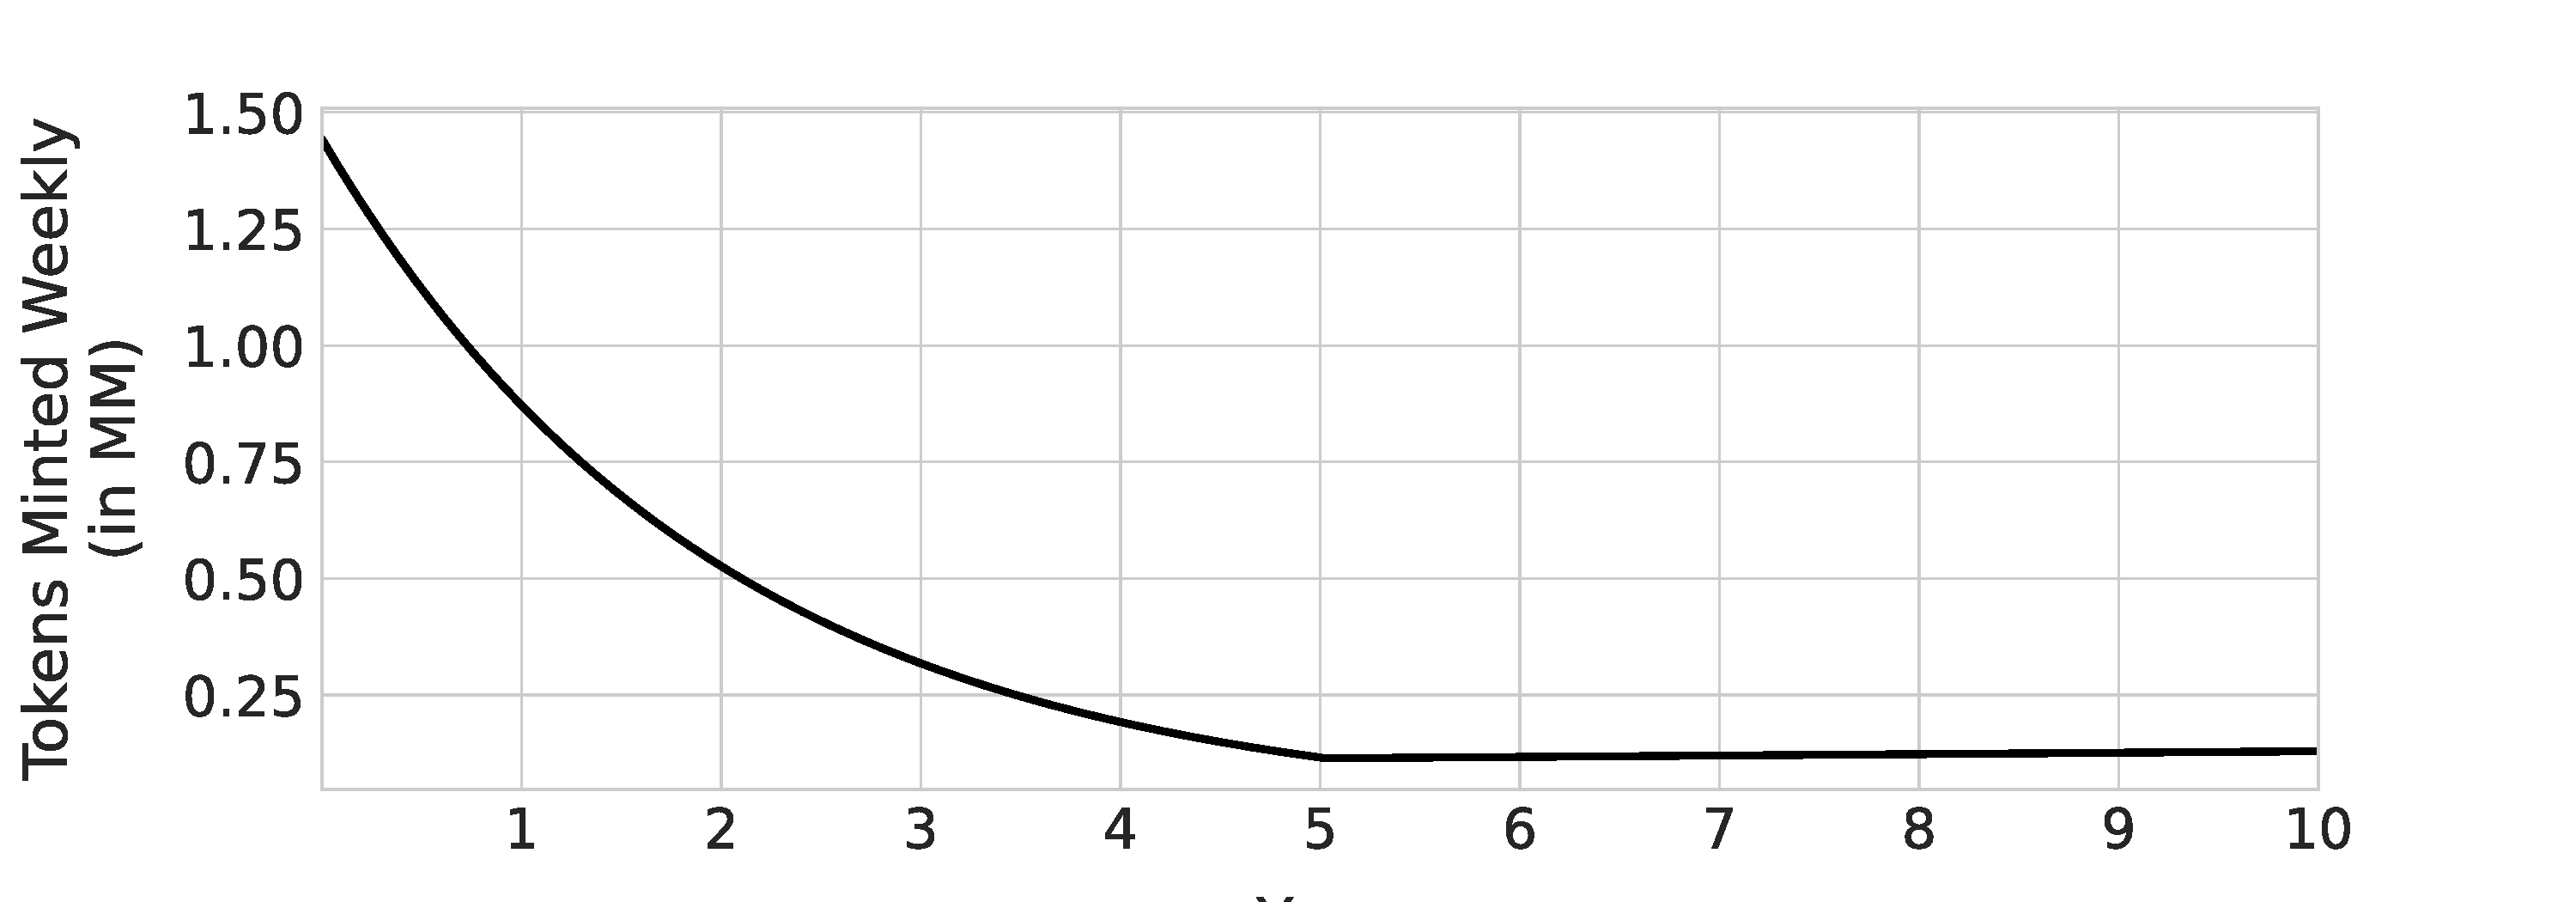
\includegraphics[width=\textwidth]{fig/token/token-weekly-emission}
         \caption{The number of tokens minted every week is exponentially decayed to reduce the annual inflation rate from $75\%$ to $2.5\%$ until the end of year 5.
         At the end of year 5, the annual inflation rate is fixed at a constant $2.5\%$.}
         \label{fig:token-emission}
     \end{subfigure}
     \begin{subfigure}{0.9\textwidth}
         \centering
         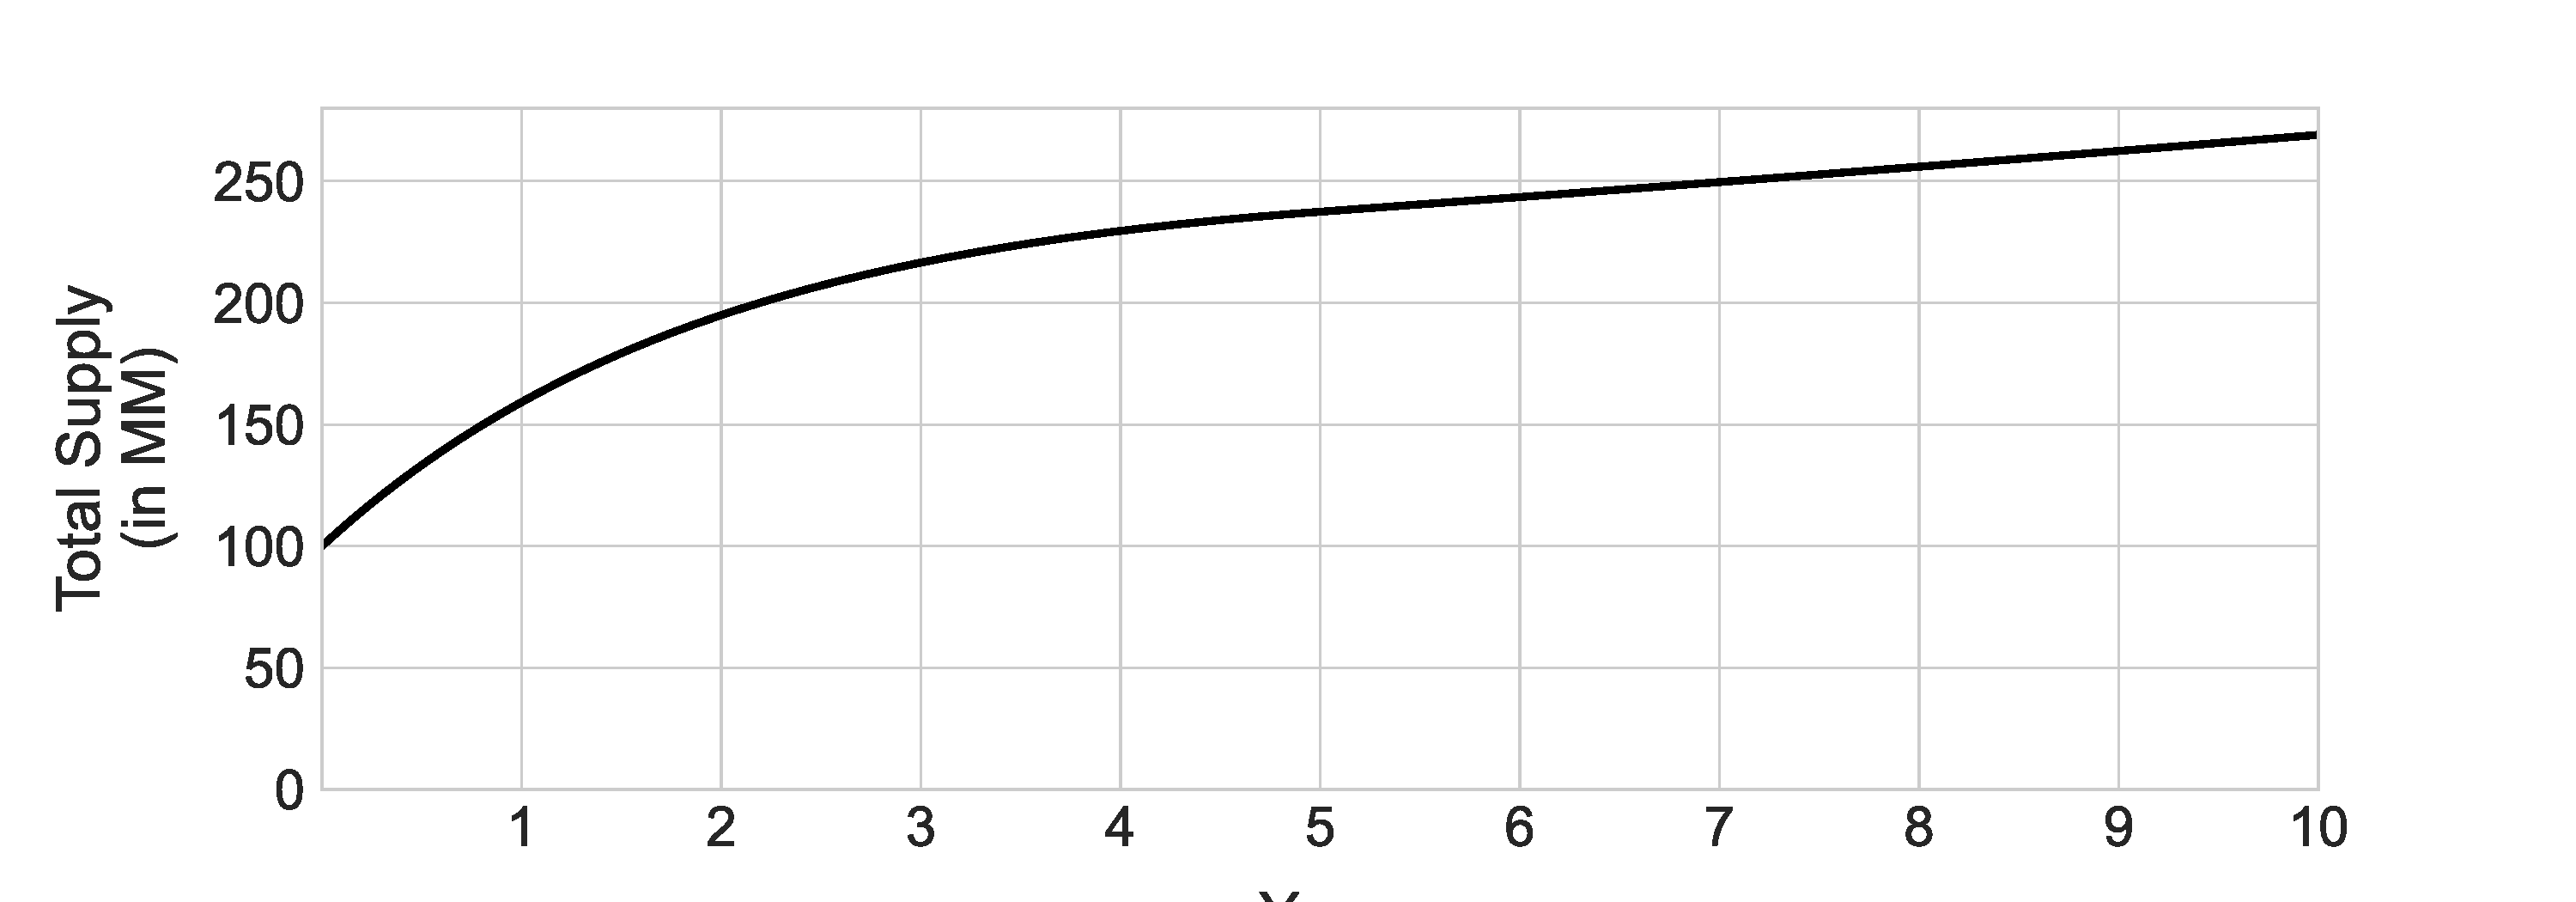
\includegraphics[width=\textwidth]{fig/token/token-total-supply}
         \caption{The total supply of API3 tokens starts from 100 million and increases according to the schedule shown above in (a).}
         \label{fig:total-supply}
     \end{subfigure}
    \caption{API3 token inflation schedule for staking rewards.}
    \label{fig:token}
\end{figure}

In essence, inflationary rewards force token holders to stake to preserve the value of their tokens.
However, staking is risky due to the funds being used as collateral, and forces the staker to participate in governance to ensure that the risk is minimized (a similar mechanic is proposed recently in~\cite{aave}).
As a combination of the two, an inflationary governance token used as collateral forces all token holders to participate in governance, which is ideal because it maximizes the decentralization of governance.
Furthermore, inflationary rewards are vested for a year, which results in governing parties sharing the project’s long term interests.

The inflationary rewards will start at a 75\% annual rate (1.44\% weekly), and the number of tokens minted weekly will be decayed exponentially until annual inflation rate becomes 2.5\% at the end of year 5.
From this point on, the annual inflation will stay at a rate of 2.5\% for perpetuity (see Figure~\ref{fig:token-emission}).
The change in the total supply of API3 tokens is illustrated in Figure~\ref{fig:total-supply}.
The proposed inflation schedule is adapted from \cite{sip-24} and will be governable.

\subsubsection{Collateral}
\label{sec:collateral}

If staking API3 only yielded rewards, the sole governance incentive would be to maximize the revenue.
This would be done by increasing the number of dAPI users aggressively, and the amount that is secured by the dAPIs with it.
In Section~\ref{sec:middleman-tax}, we have shown that the total load a dAPI is under increases its likelihood to malfunction due to an attack.
Therefore, this is not a sustainable governance strategy for decentralized data feeds.

Exposing the governing parties to the risk that we are trying to avoid would align their incentives with the DAO’s.
Then, the governing parties need to be penalized when a dAPI malfunction occurs.
We went one step further and designed an on-chain insurance service that provides dAPI users with quantifiable and trustless security guarantees.
This insurance service uses the API3 token staking pool as collateral, which means that when a dAPI malfunction is confirmed through the dispute resolution protocol, the user damages will be covered from the staking pool.
See Section~\ref{sec:quantifiable-security-through-insurance} for the details of how this insurance service will be implemented.

\begin{figure}
     \centering
     \begin{subfigure}{0.49\textwidth}
         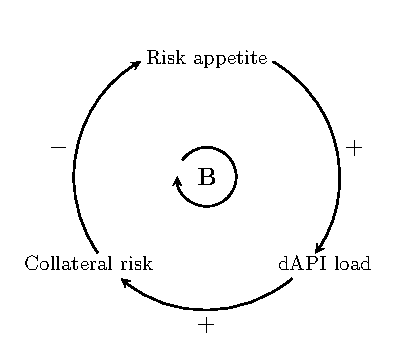
\includegraphics[width=\textwidth]{fig/systems-diagram-full/systems-diagram}
         \caption{Systems diagram of governance}
         \label{fig:systems-diagram}
     \end{subfigure}
     \begin{subfigure}{0.49\textwidth}
         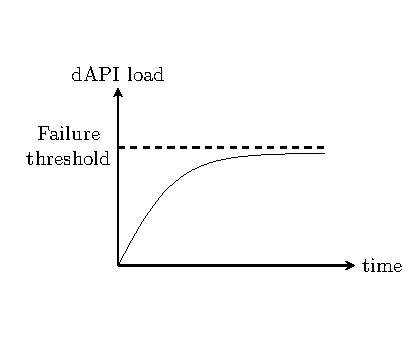
\includegraphics[width=\textwidth]{fig/systems-diagram-full/systems-diagram-plot}
         \caption{dAPI load over time in a balanced system}
         \label{fig:systems-diagram-plot}
     \end{subfigure}
    \caption{Staking and insurance collateralization utilities of the API3 token results in balanced governance incentives.
    \textbf{(a)} Loading the dAPIs with more users increases the likelihood of paying out insurance claims, which produces negative feedback and balances the system.
   \textbf{(b)} Due to the balanced nature of the system, the dAPI load does not increase indefinitely, yet settles at a level that the DAO estimates as being below the maximum load the dAPIs can support.}
    \label{fig:systems-diagram-full}
\end{figure}

Let us see the effect of using the staking pool for both collateral and governance in a systems diagram in Figure~\ref{fig:systems-diagram}.
When the DAO has appetite for additional risk, it onboards new dAPI users, which increases the load on the dAPIs.
This increases the probability of a dAPI malfunction, the likelihood of paying out an insurance claim, and the overall collateral risk as a result.
With increased collateral risk, the DAO’s risk appetite gets suppressed.
In other words, the negative feedback caused by the insurance service prevents self-destructive growth.
See Figure~\ref{fig:systems-diagram-plot} for the expected dAPI load behavior that will emerge from this.
The DAO estimates a failure threshold for the dAPIs, and onboards users to converge to this value, yet does not exceed it.
Note that in the case that the DAO overestimates this threshold, the dAPIs will malfunction and the governing parties will be punished, as their staked funds will be used to pay out the insurance claim made by the affected dAPI users.
In other words, dAPI users are protected in either case.

\subsubsection{Governance}
\label{sec:governance}

The only way to gain representation at the API3 DAO will be to stake API3 tokens in the insurance collateral pool.
As such, the governing parties will be exposed to all risks and rewards of API3, and will govern to optimize them.

Inflationary rewards and the staked governance tokens being used as collateral will create a positive feedback loop in terms of governance quality.
Initial token holders will have to stake and expose themselves to risk if they do not want to lose value to inflation.
If they misgovern and lose collateral through insurance claims, these tokens will get returned to the open market, from where they will be acquired by new governing parties.
In contrast, if initial token holders govern well and cause token scarcity in the market, the representation distribution will be protected.
In other words, governance tokens being used as collateral results in a robust Darwinian structure that improves itself and is able to recover from failures.

%~~~~~~~~~~~~~~~~~~~~~~~~~~~~~~~~~~~~~~~~~~~~~~~~~~~~~~~~~~~~~~~~~~~

\section{Quantifiable Security through Insurance}
\label{sec:quantifiable-security-through-insurance}

API3 will provide dAPI users with a quantifiable level of security in the form of an on-chain insurance service.
This accomplishes two goals: (1) the insurance acts as a well-defined and trustless safety net for the user in case of a dAPI malfunction, (2) it holds the governing parties responsible for dAPI malfunctions, and thus incentivizes them to govern towards more secure dAPIs.

\subsection{The need for quantifiable security}
\label{sec:the-need-for-quantifiable-security}

\begin{quote}
\it
    Engineering is the art of modelling materials we do not wholly understand, into shapes we cannot precisely analyse, so as to withstand forces we cannot properly assess, in such a way that the public has no reason to suspect the extent of our ignorance.
\end{quote}
\begin{flushright}
-- Dr. A. R. Dykes
\end{flushright}

If we asked an engineer ``How much load can your bridge support?'' and got the answer ``I can assure you it has 21 beams of highest quality steel,'' we would not want to use that bridge, since not being able to provide the maximum load is an engineering red flag.
We have introduced a simplistic model for how much a single oracle and, by derivation, a data feed would be able to support in Section~\ref{sec:middleman-tax}.
While not exhaustive, this model demonstrates that decentralized oracle networks cannot secure an arbitrarily large monetary value.
The amount safely secured by an oracle must be bounded.
In other words, like all blockchain technology, decentralized oracle networks should only be trusted to a certain extent, rather than being treated as unconditionally trustless~\cite{defilippi:2020}.
Then, a data feed---centralized~\cite{coinbase} or decentralized~\cite{ellis:2017}---should be responsible for quantifying the amount it can secure.

One of the most well recognized solutions to this issue is proposed for the UMA protocol~\cite{uma:2020}.
The proposed scheme not only allows the quantification of the amount that can be secured by a data feed using game theoretic principles, it also allows this limit to be set precisely.
The authors astutely observe that an overly-secure data feed is not desirable because it will be unnecessarily expensive for its users, and being able to set the degree of security to the minimum requirements would reduce costs.
However, they follow this with the claim that the method they have proposed is optimally cost-efficient, which is grossly inaccurate in practice.
This mistake stems from approaching the problem in a data source-blind way, i.e., trying to solve the oracle problem instead of the API connectivity problem.
The proposed solution is only optimally cost-efficient if we consider all oracles to be untrustworthy, which is a close enough approximation for third-party oracles.
In contrast, the trustworthiness of first-party oracles can be leveraged to build extremely secure data feeds at a very low cost, as the API providers have too much to lose by attempting an attack.
A high value DeFi product being successfully secured by the data provided by a single reputable centralized exchange demonstrates this fact very well~\cite{coinbase}.
Therefore, one cannot hope to disregard substantiated trustworthiness and end up with an actually cost-efficient solution.

The ideal solution that fits the API3 vision must provide quantifiable security guarantees by drawing from the trustworthiness of API providers, which can only be assessed using off-chain information.
To achieve this, API3 will provide an insurance service that guarantees to a dAPI user that damages due to a malfunction will be covered up to a predetermined amount.
This solution is preferable for the user, as an alternative game theoretic solution can unexpectedly fail due to incentives that are poorly modeled or unaccounted for.

\subsection{dAPI Insurance}
\label{sec:dapi-insurance}

In Section~\ref{sec:centralized-oracle-network-governance}, we mentioned a security incident where a Chainlink data feed had misreported to Synthetix.
This was reported to cause damages less than \$40,000 by Chainlink on the day of the incident~\cite{chainlink-fatfinger} and approximately \$36,000 by Synthetix the day after~\cite{synthetix-fatfinger}.
Furthermore, Synthetix then announced that Chainlink had offered to compensate the damages, which they have subsequently accepted.
This incident has demonstrated the following:

\begin{enumerate}
    \item Insurance that pays for damages is a natural and obvious solution to data feed malfunction.
    \item It is generally understood that the governing entity is responsible for data feed malfunctions.
    \item It is possible to determine data feed malfunctions, their causes, and the resulting damages in a matter of days.
\end{enumerate}

On the surface, this incident was resolved rather uneventfully.
This is to be expected, as the amount in question was relatively insignificant to the respective parties.
However, neither the general public nor the stakeholders can be sure of the exact terms of the settlement, as both projects are governed in a centralized way.
This leads us to ask: What would have happened if the damages were orders of magnitude larger?
How are fully decentralized projects supposed to deal with such events?

It has been shown that insurance usage not only correlates with macroeconomic growth, but is also a cause of it~\cite{outreville:2013}.
Nevertheless, insurance is sorely underutilized in the blockchain space.
One of the main reasons of this is that insurance naturally requires a third party to resolve insurance disputes, and using a mutually-trusted third party for this purpose is against the ethos of decentralization.
However, the emergence of Kleros~\cite{kleros:2019}, a general purpose on-chain dispute resolution protocol, allows trustless insurance products to be built.

API3 will co-develop an on-chain insurance service with Kleros that provides quantifiable and trustless security guarantees to dAPI users.
This insurance service will protect the dAPI user against damages caused by certain dAPI malfunctions up to a payout limit.
Note that even if we did not provide this service, the dAPI user could have received on-chain insurance services using a third party solution~\cite{nexus-mutual}.
Such a solution would tend towards charging very high insurance premiums, as they would not have access to the information and expertise to accurately assess dAPI risks.
Furthermore, as described in Section~\ref{sec:collateral}, the proposed insurance service is special in the way that it is collateralized by the funds staked by the governing parties of the API3 DAO.
Therefore, it not only provides security guarantees to the dAPI user, but also creates a very strong incentive for dAPIs to be governed in a way that their security is maximized, which will further decrease insurance costs.

\subsection{Insurance process}
\label{sec:insurance-process}

The user requests to subscribe to a dAPI and receive a specific insurance coverage for the respective service through off-chain channels.
The total amount that can be covered is limited by the size of the collateral pool, and the DAO will govern the collateralization ratio based on existing insurance solvency literature~\cite{solvency}.
Respective API3 teams investigate the dAPI malfunction risks and the specific use case of the user, calculate the insurance premium, and enter the user-specific fee to the contract that manages payments.
Upon paying the fee to the contract, the dAPI user gains access to the dAPI and gets insured for the respective payment period.

If the dAPI user notices a malfunction, they will assess damages and make an on-chain insurance claim.
This will automatically lock the claimed amount at the collateral pool described in Section~\ref{sec:api3-tokenomics}.
Stake withdrawals will have an adequate lead-time that will prevent stakers from front-running claims, i.e., withdrawing as soon as a dAPI malfunctions to evade claims.
On the other hand, the insuree will need to stake funds to be able to make a claim to disincentivize abuse.
The API3 DAO can either pay out the claim directly, or escalate the claim to the Kleros court, which will determine if the claimed amount will be paid out to the dAPI user.
The claim being denied will result in the tokens being unlocked, while the claim being accepted will result in the tokens being transferred to the dAPI user.
This corresponds to stakers covering the damages proportional to the amount they have staked; that is, a user who has staked tokens that make up $p\%$ of the entire pool will pay $p\%$ of an accepted claim.

The scheme described above assumes all amounts to be denominated in API3 tokens.
Depending on the use case, some users may require to be insured in other cryptocurrency types, e.g., ETH.
In this case, simply having a liquidity provider automatically convert the payout to ETH will not be enough, as the API3/ETH exchange rate between the time the claim is made and it is paid out will change, resulting in slippage.
As a solution, the API3 DAO can maintain an additional ETH reserve---subject to the same solvency considerations as the collateral pool---to absorb the price volatility and ensure that the payout meets the amount that the user has originally claimed.

\subsection{Risk Assessment}
\label{sec:risk-assessment}

Quantifying the amount of security that a data feed can provide is a very difficult problem.
However, by embedding the problem into the established domain of insurance, we gain access to a wide variety of literature and skills that are readily available to source from traditional insurance services.
Therefore, API3 will be well-equipped with the services of actuaries, statisticians, data scientists, rate-makers, analysts, and legal counsel in taking on the challenging task of providing quantifiable security guarantees.

Risk assessment is a vital step in optimizing insurance pricing and making correct solvency estimations.
This includes two main factors:
\begin{itemize}
    \item Internal: How likely is it for the dAPI to malfunction?
    \item External: What is the expected value of damages caused by a possible dAPI malfunction?
\end{itemize}

One of the most important internal risk factors here is failure at the oracle level, which can be estimated by investigating individual APIs qualitatively, and analyzing their performance statistically.
For example, qualitative investigations may conclude that an API provider has been in business for 5 years, and thus does not constitute a significant Sybil attack risk.
Similarly, statistical analysis may indicate that the data provided from an API provider often diverges from the consensus, which may cause an issue if the data consumer demands high accuracy.
These assessments will also provide guidance in designing dAPIs regarding the number and selection of the API providers, e.g., it can be found out that adding more APIs to an overloaded dAPI will end up reducing costs by decreasing the insurance risk.
Operational risks are another important factor, which can be assessed through audits that investigate operational processes.
Note that since this research will be done by the API3 teams and publicly reported to the DAO, it will provide unmatched transparency and security assurance to the users.

\begin{figure}[!t]
     \centering
     \begin{subfigure}{0.38\textwidth}
         \centering
         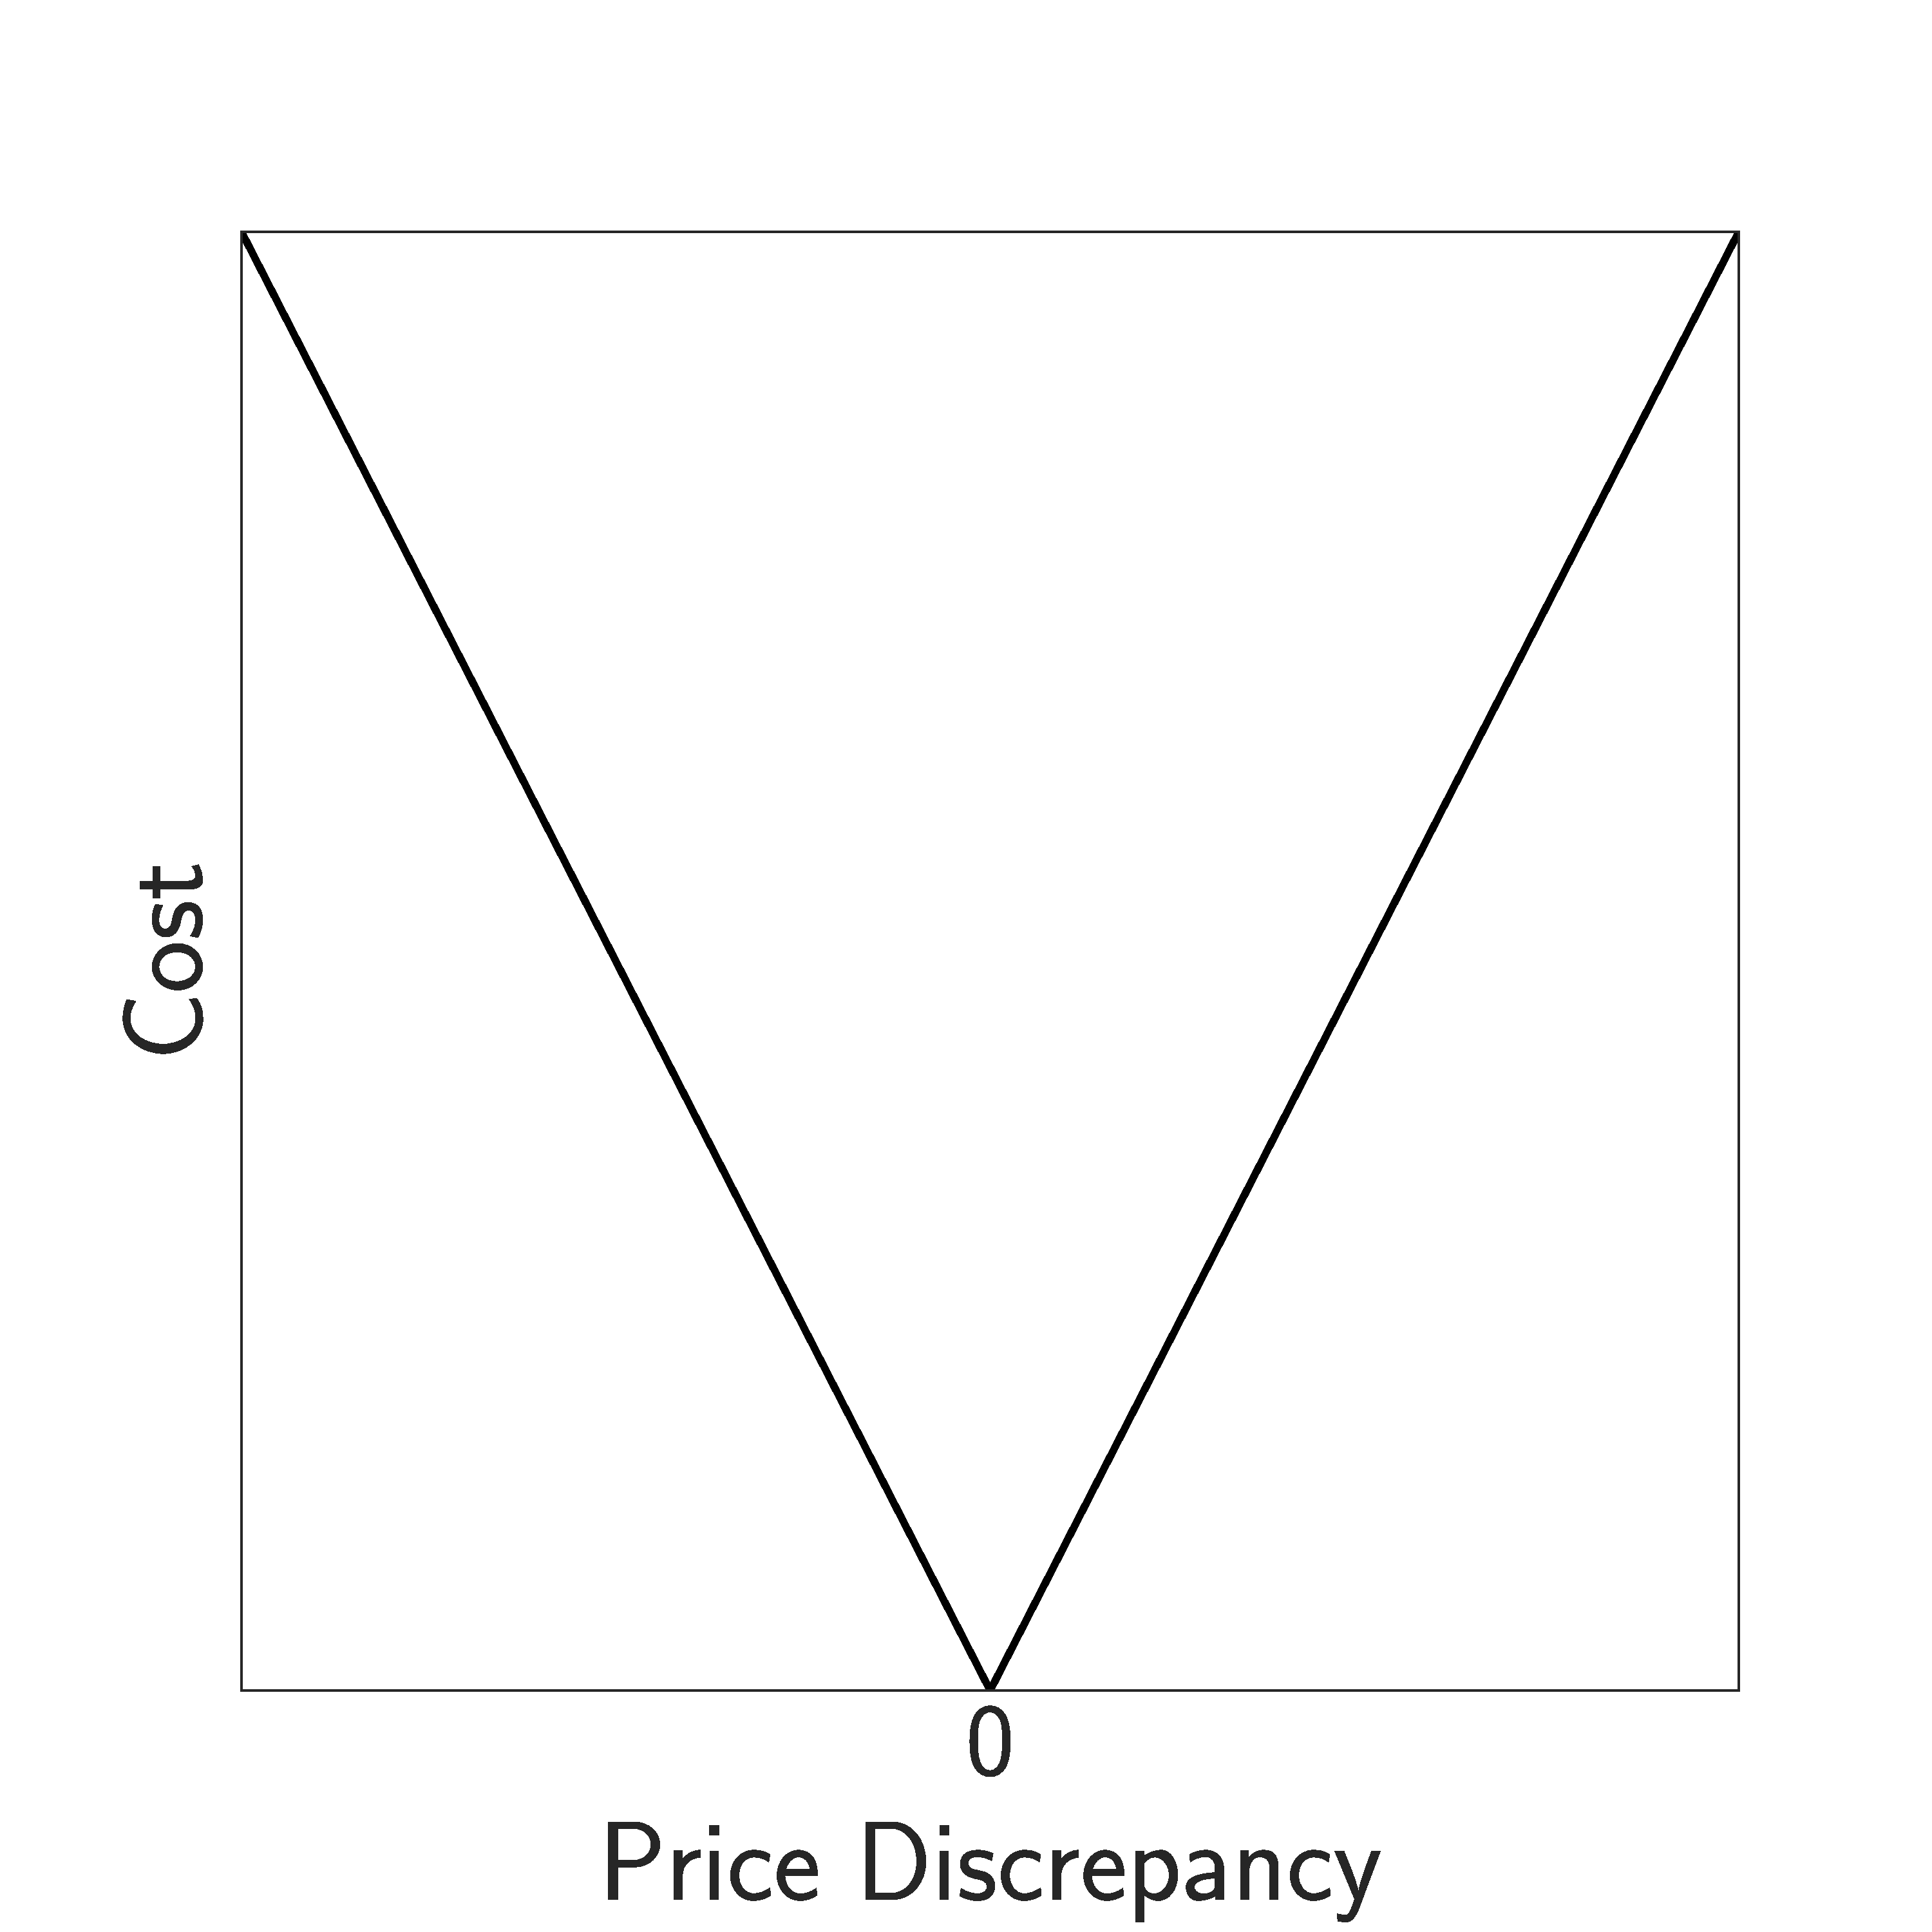
\includegraphics[width=\textwidth]{fig/use-case-types/use-case-linear}
         \caption{linear}
         \label{fig:use-case-linear}
     \end{subfigure}
     
     \begin{subfigure}{0.38\textwidth}
         \centering
         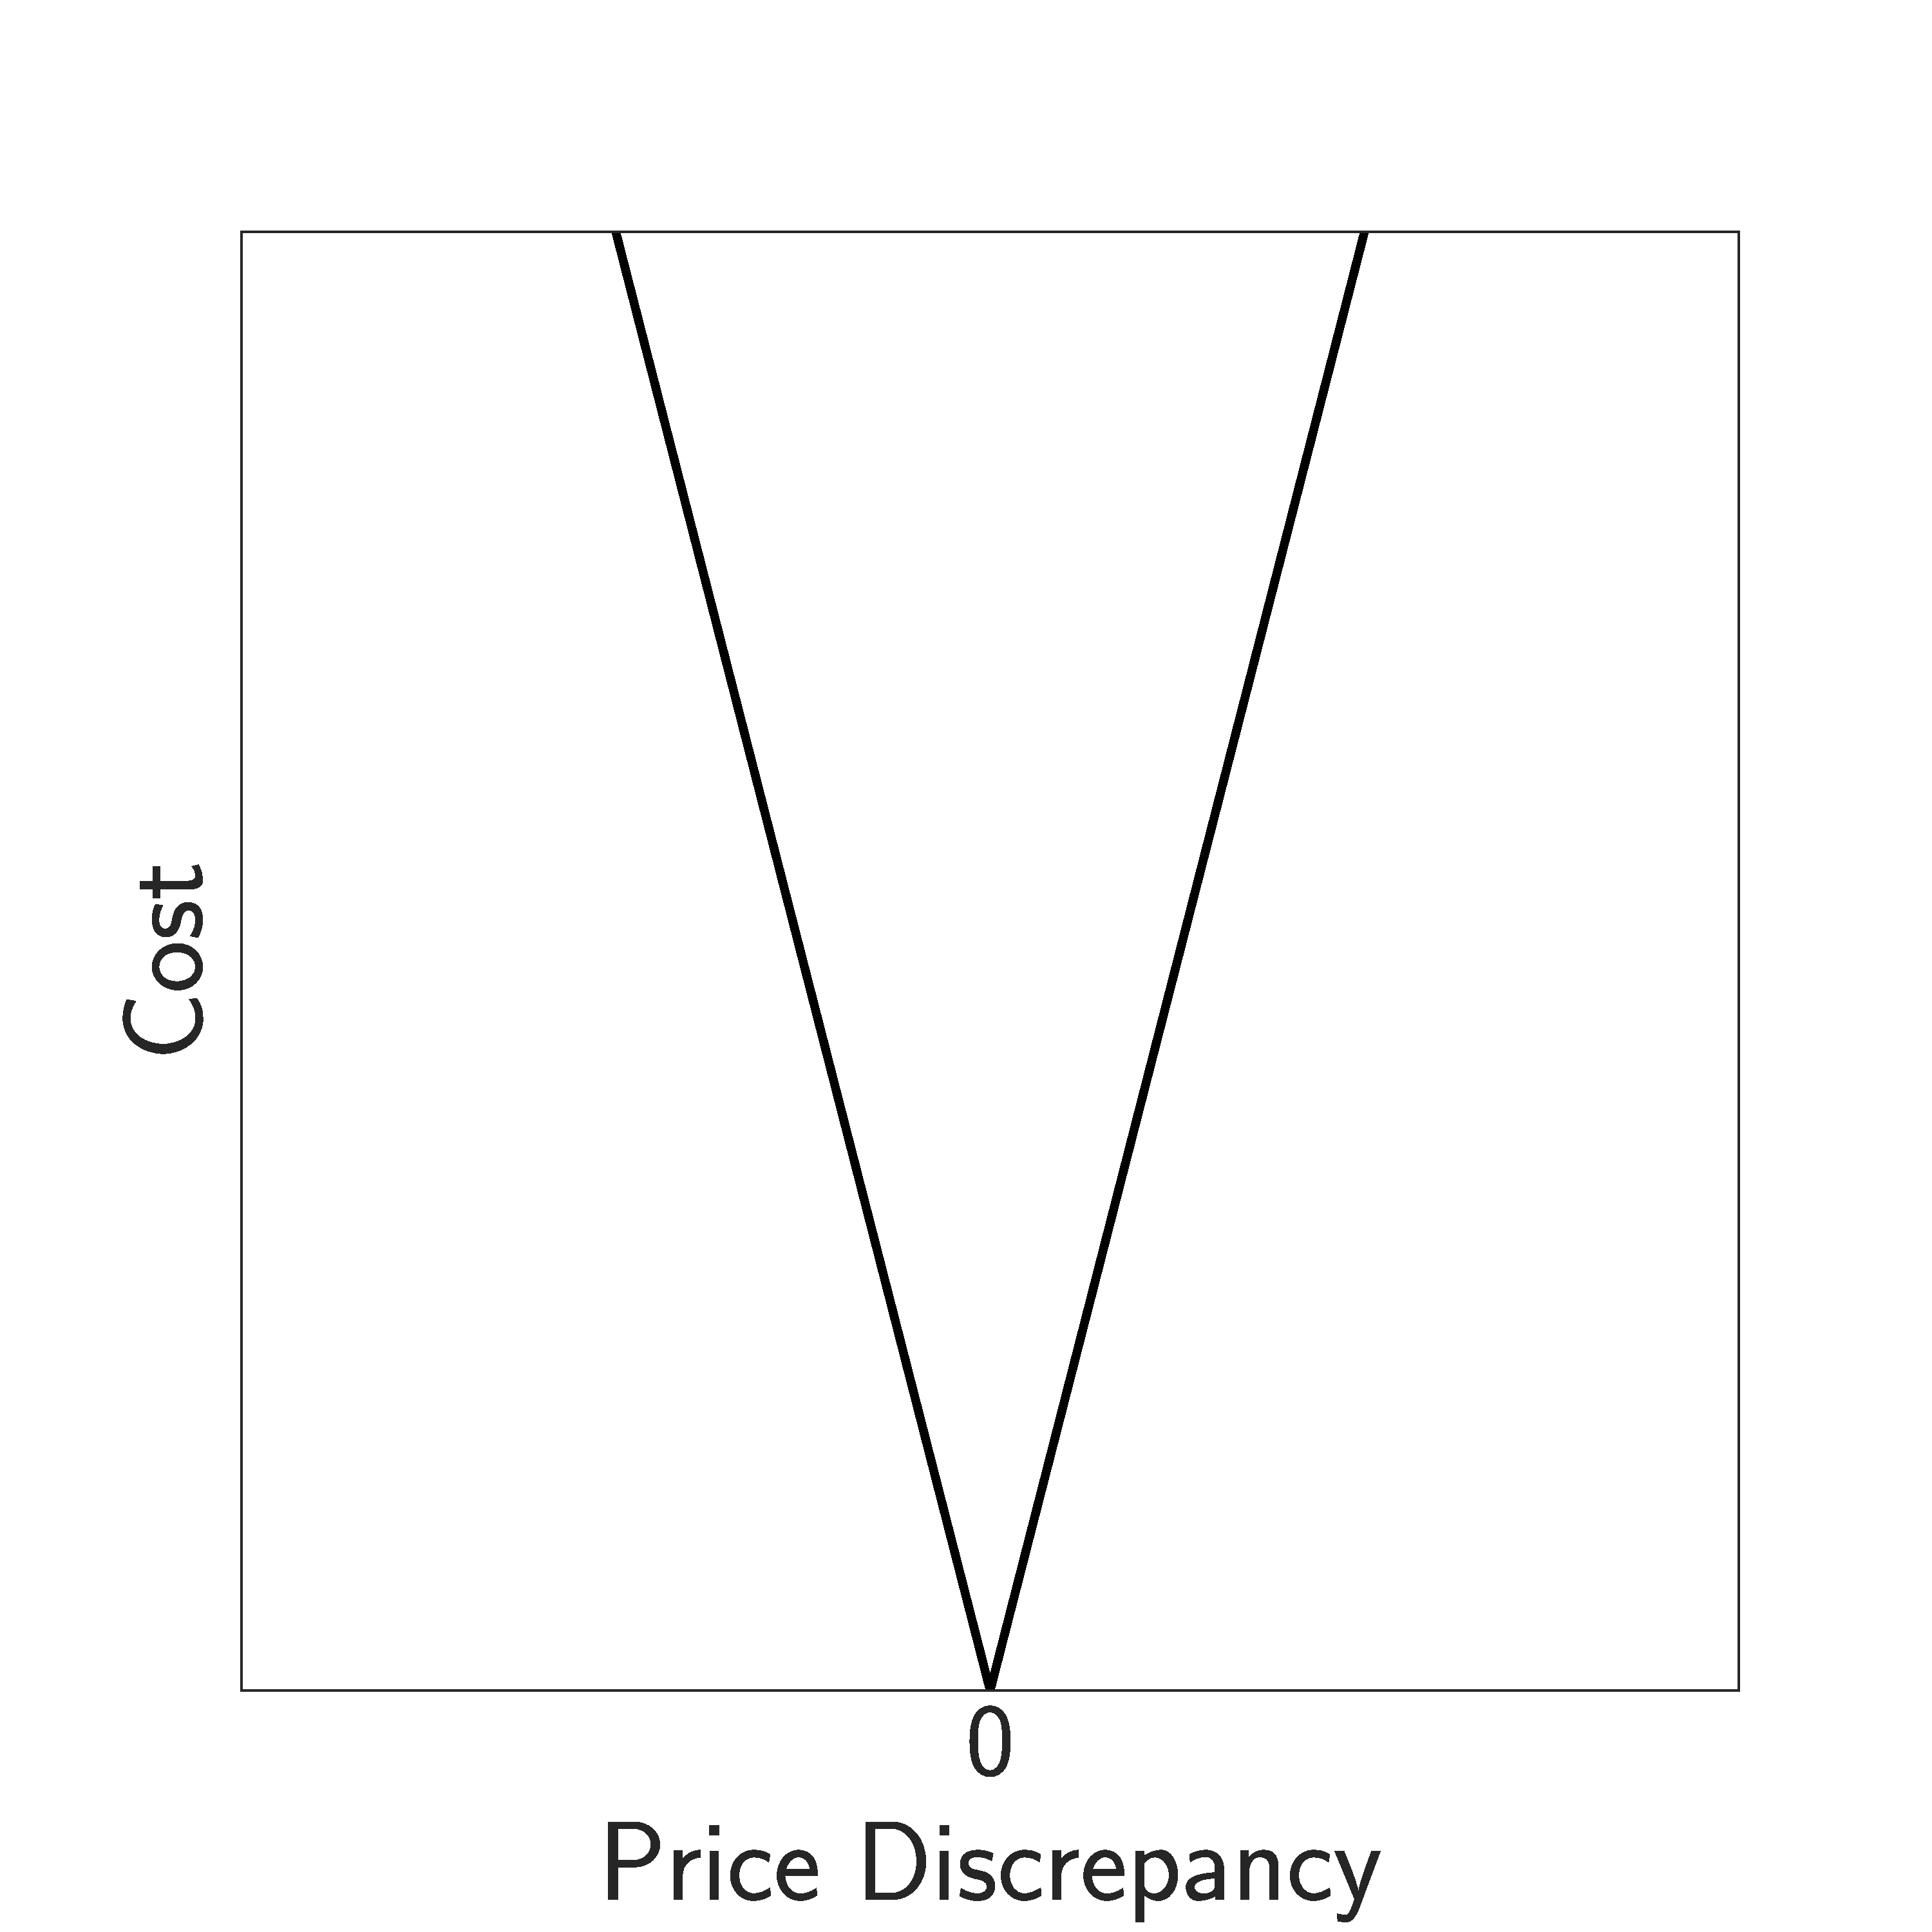
\includegraphics[width=\textwidth]{fig/use-case-types/use-case-leveraged}
         \caption{leveraged}
         \label{fig:use-case-leveraged}
     \end{subfigure}
     \begin{subfigure}{0.38\textwidth}
         \centering
         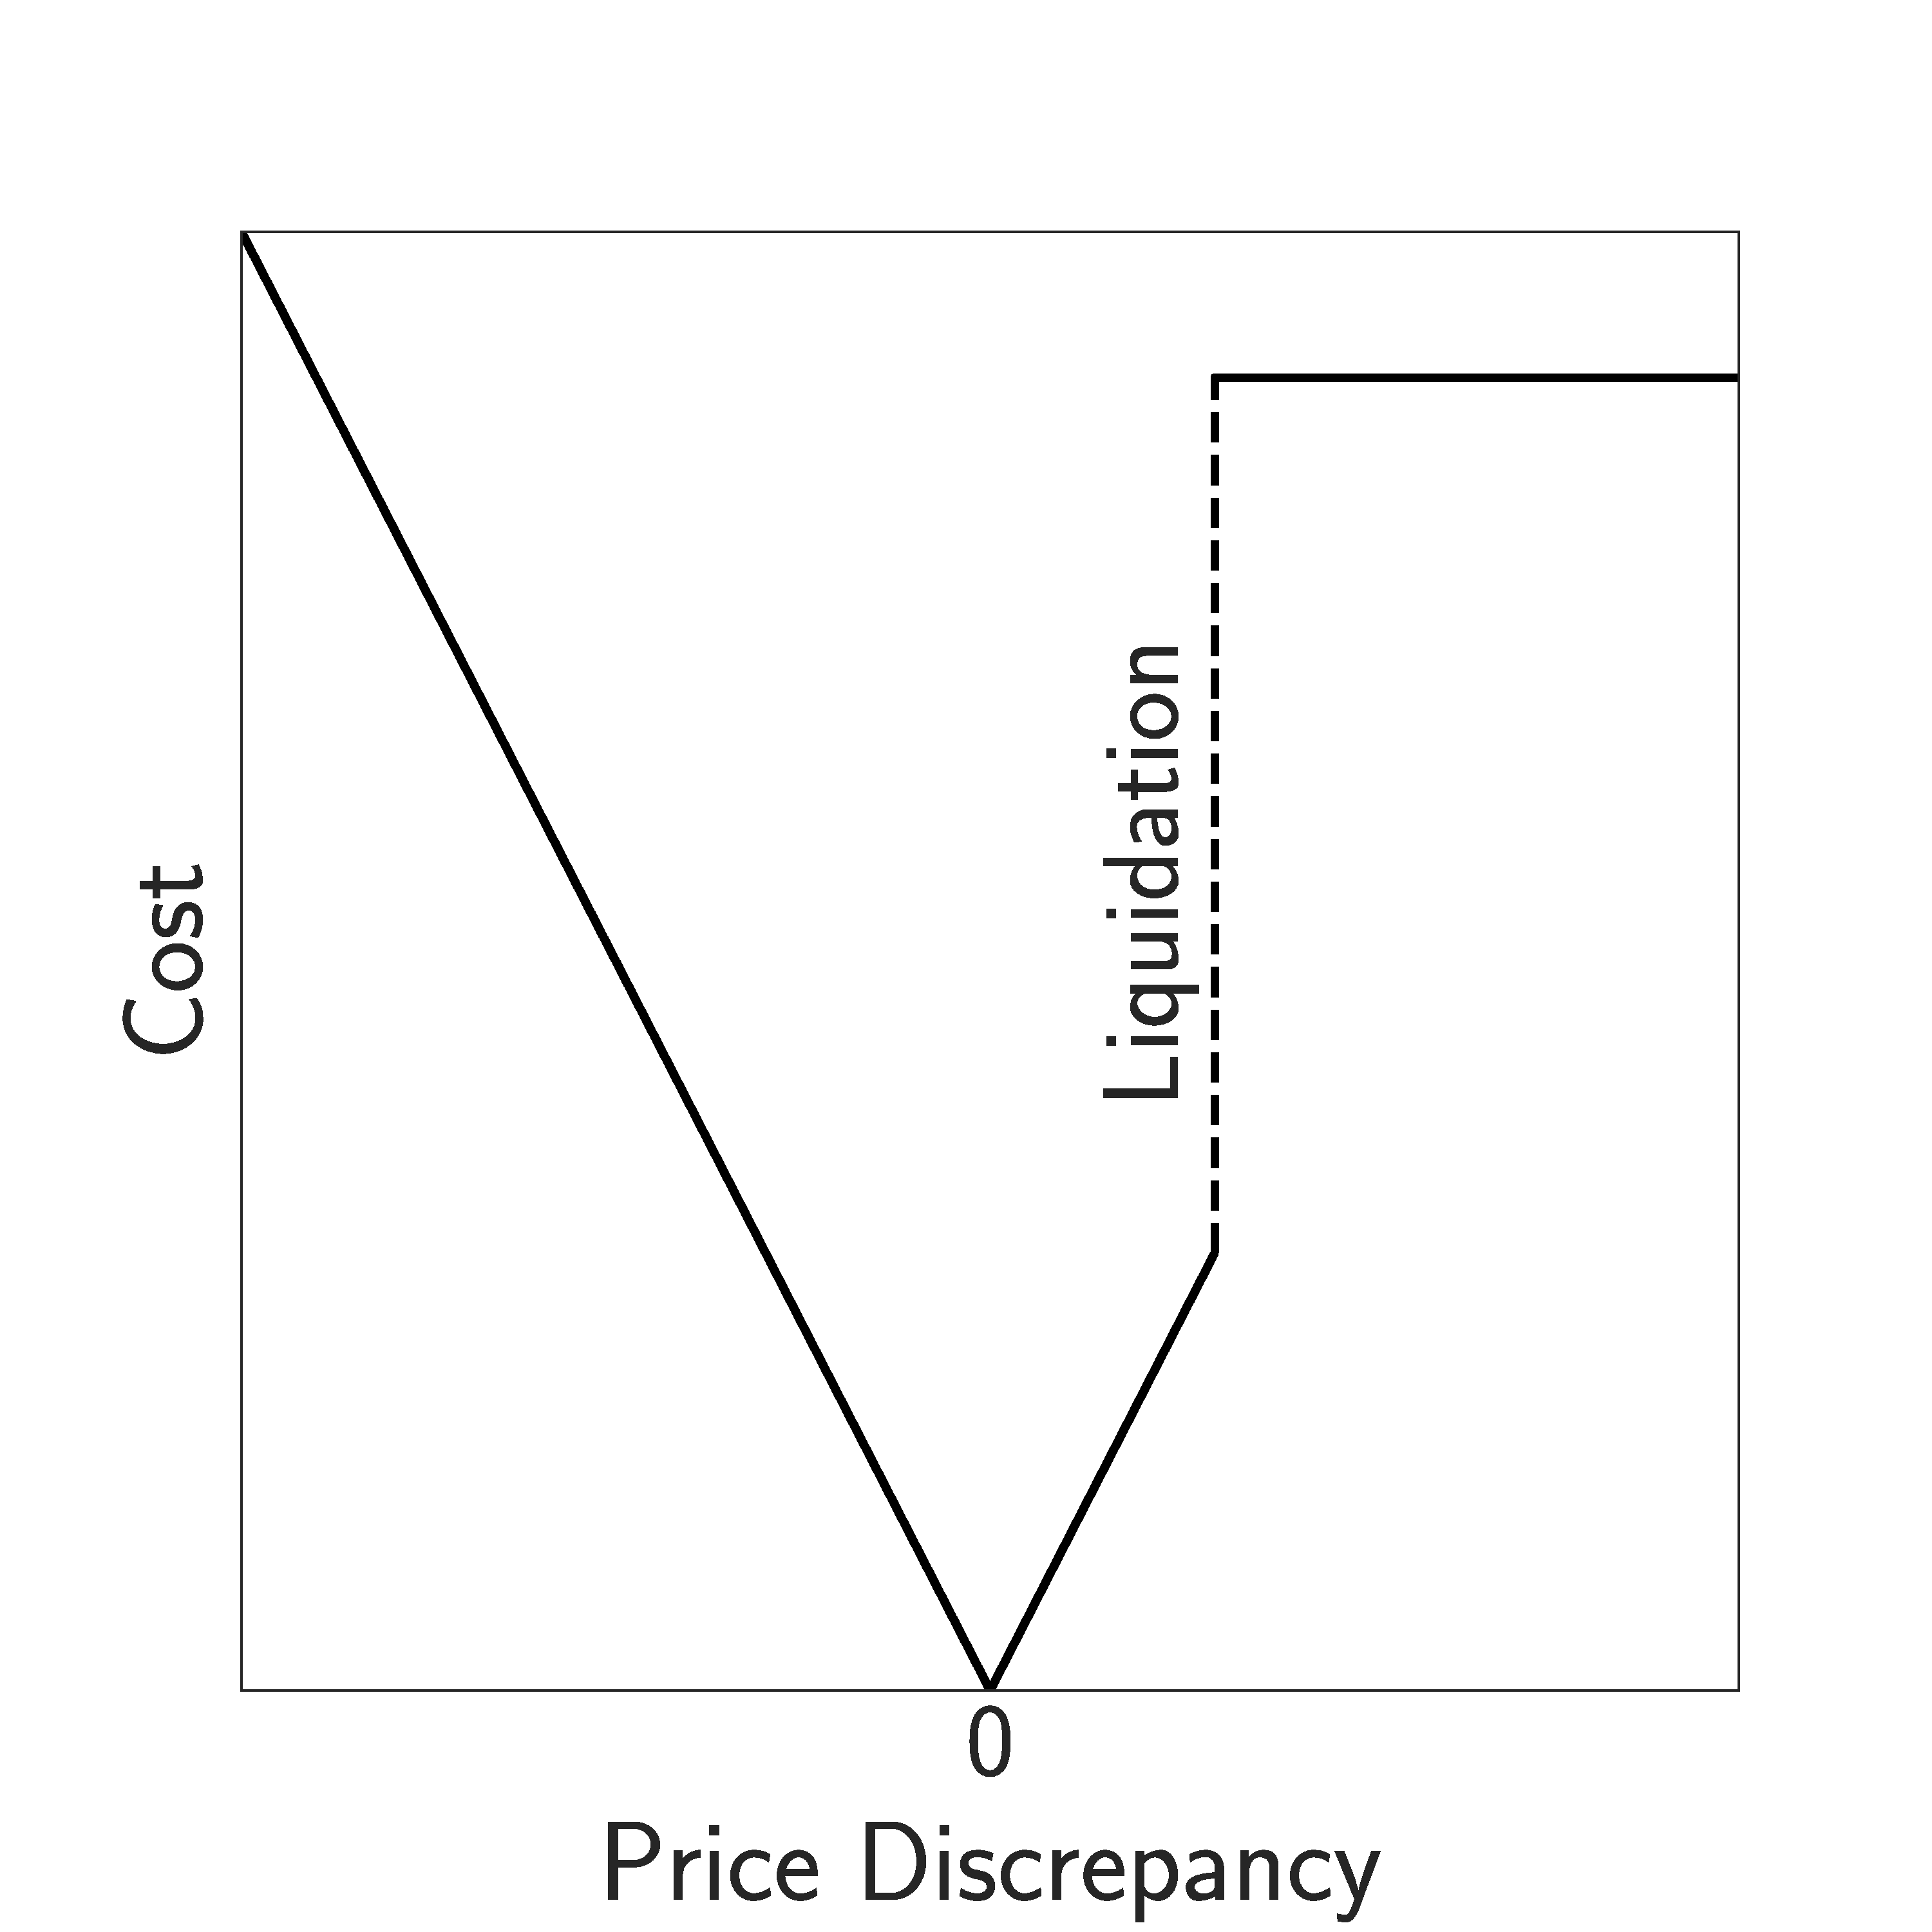
\includegraphics[width=\textwidth]{fig/use-case-types/use-case-discontinuous}
         \caption{discontinuous, e.g. liquidation}
         \label{fig:use-case-discontinuous}
     \end{subfigure}
    \caption{The data from the dAPI can be used in different systems, and the linearity and continuity in the mechanics of these systems decide on how sensitive they are to errors in input data.}
    \label{fig:use-case-types}
\end{figure}

External risk factors determine the expected value of damages when a malfunction happens, and how the data is being used is an important aspect of this.
See Figure~\ref{fig:use-case-types}, where we illustrate the cost of data errors for various hypothetical DeFi applications.
In Figure~\ref{fig:use-case-linear}, the dAPI provides price data to a regular exchange, and errors result in a linearly proportional profit and loss for the transacting parties (note that we only consider the losses).
Compare this with Figure~\ref{fig:use-case-leveraged}, which represents an exchange with a similar volume that supports leveraged positions.
Here, any misreport has a much larger potential to cause damages.
Finally, see Figure~\ref{fig:use-case-discontinuous}, where a user has opened a short position.
A slight skew upwards in the reported data may trigger a liquidation and cause a disproportionate effect.
These examples indicate that it is impossible to estimate the insurance risk for a specific user without considering how exactly they will use the data they receive from the dAPI.

There is also a more qualitative aspect of the insurance.
Specifically, API3 and the dAPI user will agree on an insurance policy, which defines terms such as what a dAPI malfunction is and how damages are calculated.
Kleros jurors will be using these policies as reference while deciding if an insurance claim is to be paid out.
The specific terms are important regarding how insurance rates are to be determined.
For example, insurance that covers any malfunction would be more expensive than insurance against downtime.

\subsection{Scaling solutions and insurance}
\label{sec:scaling-solutions-and-insurance}

High value use cases such as DeFi becoming popular causes the Ethereum network to be congested.
This increases the transaction fees and affects data feed operation costs as a result.
Then, it becomes critical to be able to make use of scaling solutions to deliver dAPI services at a reasonable cost.

Existing decentralized oracle solutions propose to use off-chain scaling solutions~\cite{ellis:2017,band}.
However, these solutions come with obscure security implications that the user cannot assess accurately.
Firstly, scaling solutions tend to have more relaxed security guarantees in general, and it is not reasonable to expect the user to have a solid understanding of the consequences.
Furthermore, there are additional operational risks, e.g., security issues with the implementation of a custom cryptographic function, the second layer solution denying service, etc.
As a result, it would be reasonable to expect users to be apprehensive about using data feeds depending on scaling solutions.

dAPI insurance comes as an unexpected solution to this problem due to its flexibility.
If the API3 DAO decides that a scaling solution is reasonably trustworthy for a given use case, the respective dAPI can utilize that scaling solution, and its insurance would cover potential damages that would be caused by the scaling solution.
The entire insurance claims process would work exactly the same, given that what ultimately matters is whether or not the service is correctly delivered to the dAPI user.

\section{Conclusion}
\label{sec:conclusion}

API3 will connect decentralized applications with the abundant data and services offered by traditional Web APIs, thereby expanding the applicability of the blockchain without sacrificing decentralization.
This will be achieved by dAPIs---fully decentralized and blockchain-native APIs---which will be set up, managed, and monetized at scale by the API3 DAO.

The API3 solution embodies a variety of qualities by design.
The most important one among these is \textbf{security}. dAPIs do not depend on third-party oracles, which are a constant and significant risk factor in the alternative solutions.
In addition, the dAPI insurance service provides quantifiable and trustless security guarantees to its users, further cementing API3’s place as the most secure solution to receiving API services as a decentralized application.

The second quality of the API3 solution is \textbf{robustness} on multiple levels.
Airnode uses serverless technology, which is highly resistant against downtime.
Paired with a stateless node design that is not easily affected by bugs or adverse network conditions, API3 oracles are engineered for robustness.
Moreover, the dAPIs will be governed by a DAO that maintains a self-regulating balance of risk and reward through well-engineered incentives, which provides a robust risk mitigation framework.

dAPIs eliminate the middlemen, which grants them their third quality, \textbf{cost-efficiency}.
They do not have to pay the middleman tax, which is the payment made to third-party oracles to incentivize them against attempting an attack.
In addition, data feeds composed of first-party oracles do not require over-redundancy at the oracle level.
By achieving the same level of decentralization with fewer oracles, dAPIs provide very significant savings in gas costs.

Finally, the API3 solution achieves \textbf{flexibility} through complete decentralization of governance to parties with real skin in the game.
As a result, the project will never be limited by what is put forth in this paper, and will evolve constantly to meet new challenges and needs.

The first generation of decentralized applications were limited to the confines of the blockchain.
Today, we have decentralized applications that can interact with the off-chain world in a limited and pseudo-decentralized way.
API3 will power the next evolutionary wave---the third generation of decentralized applications that valuably interact with the off-chain world, leveraging APIs in a truly decentralized and trust-minimized way.

\small
\bibliographystyle{ieeetr}
\bibliography{refs}

\newpage
\normalsize
\appendix
\section{Glossary}

\textbf{Airnode:} A fully-serverless oracle node designed to be operated by API providers.

\textbf{API:} A technical interface of an application that another application can use to interact with it programmatically.
An API that is open to external access (i.e., a Web API) can be used by businesses to monetize their data and services.

\textbf{API provider:} A business that monetizes their data and services through an API.

\textbf{API3:} The project that will build, manage, and monetize dAPIs.

\textbf{API3 DAO:} The governing body of the API3 Project.

\textbf{API3 token:} The token that is used to align the API3 ecosystem incentives.
It grants voting power at the API3 DAO.

\textbf{ChainAPI:} A third-party API--Airnode integration platform.
It will provide integration tools, utilities and a marketplace for public listing of oracle endpoints.
It can be thought of as the spiritual successor to the Honeycomb API Marketplace.

\textbf{DAO:} Decentralized autonomous organization.
A multi-user smart contract that is used to democratize the governance of an on-chain organization.

\textbf{dAPI:} A decentralized API, i.e., a data feed composed of first-party oracles.
It is governed decentrally by the API3 DAO.

\textbf{Honeycomb API Marketplace:} An API-centric marketplace/listing service that has been built for Chainlink oracles by some of the founding members of API3.

\textbf{Oracle:} An agent that can deliver data to-and-from a smart contract platform, e.g., writes asset price data to the chain.
It includes a node and a smart contract that implements the protocol it uses to communicate with the requesters.

\textbf{Oracle node:} An application that performs the off-chain functions of an oracle, e.g., calls an API to get asset price data and writes it to the chain.

\textbf{Web 3.0:} The decentralized Web built over blockchain technologies.
Note that we are not using this term to refer to the Semantic Web.

\textbf{Web API:} An API that is accessible over the Web, i.e., an API that is not only accessible from a private network.

\end{document}
